\documentclass[a4paper,11pt]{report}
\usepackage[showexo=true,showcorr=false]{../packages/coursclasse}
%Commenter ou enlever le commentaire sur la ligne suivante pour montrer le niveau
\toggletrue{montrerNiveaux}
%permet de gérer l'espacement entre les items des env enumerate et enumitem
\usepackage{enumitem}
\setlist[enumerate]{align=left,leftmargin=1cm,itemsep=10pt,parsep=0pt,topsep=0pt,rightmargin=0.5cm}
\setlist[itemize]{align=left,labelsep=1em,leftmargin=*,itemsep=0pt,parsep=0pt,topsep=0pt,rightmargin=0cm}
%permet de gerer l'espacement entre les colonnes de multicols
\setlength\columnsep{35pt}
\let\oldcenter\center
\let\oldendcenter\endcenter
\renewenvironment{center}{\setlength\topsep{-10pt}\oldcenter}{\oldendcenter}


\begin{document}
%%%%%%%%%%%%%%%%% À MODIFIER POUR CHAQUE SERIE %%%%%%%%%%%%%%%%%%%%%%%%%%%%%
\newcommand{\chapterName}{Grandeurs et mesures}
\newcommand{\serieName}{Périmètre et aire de polygones}


%%%%%%%%%%%%%%%%%% PREMIERE PAGE NE PAS MODIFER %%%%%%%%%%%%%%%%%%%%%%%%
% le chapitre en cours, ne pas changer au cours d'une série
\chapter*{\chapterName}
\thispagestyle{empty}

%%%%% LISTE AIDE MEMOIRE %%%%%%
\begin{amL}{\serieName}{

\item Hauteurs d'un triangle et orthocentre (page 117)
\item Quadrilatères particuliers (page 123)
\item Unités de longueur (page 156)
\item Unités d'aire (page 157)
\item Périmètre des surfaces usuelles (page 164)
\item Aire des surfaces usuelles (pages 165 à 167)
\item Calculer l'aire d'une figure (pages 168 et 169)
}
\end{amL}
%%%%%%%%%%%%%%% DEBUT DE LA SERIE NE PAS MODIFIER %%%%%%%%%%%%%%%%%%%%%%%%%%%%%
\section*{\serieName}
\setcounter{page}{1}
\thispagestyle{firstPage}



%%%%%%%%%%% LES EXERCICES %%%%%%%%%%%%%%%%%%%%%%%%%%%%%%%%%%%




%-----------Périmètres et aires de carrés-rectangles----------------------

\begin{resolu}{Calculer le périmètre d'un polygone}{
		Calcule le périmètre d'un rectangle qui a $\tunit{2}{cm}$ de longueur et $\tunit{5}{mm}$ de largeur.

Démarche :
\begin{tasks}
    \task Vérifie que toutes les longueurs sont exprimées dans la même unité. Si nécessaire, effectue des conversions.
    
    {\color{blue} Je convertis mes longueurs en \tunit{}{mm} : $\tunit{2}{cm}=\tunit{20}{mm}$}
    
    \task Si l'énoncé ne propose pas de croquis, dessine le polygone d'après les indications de l'énoncé. Indique toutes les grandeurs connues. 
    \begin{center}
            \begin{tikzpicture}
                \draw[color=blue] (0,0) rectangle (2,1) ;
                \node[color=blue] at (1,-0.4) {$20$} ;
                \node[color=blue] at (2.6,0.5) {$5$} ;
            \end{tikzpicture}
    \end{center}
    \vspace{-0.8cm}
    \task Identifie les longueur qui forment le contour du polygone. Utilise un crayon de couleur pour le mettre en évidence.
    \begin{center} 
            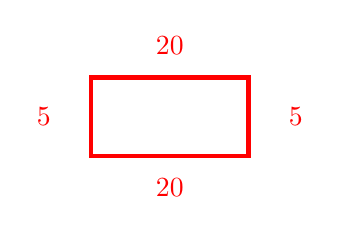
\begin{tikzpicture}
                \draw[ultra thick, color=red] (0,0) rectangle (2,1) ;
                \node[color=red] at (1,-0.4) {$20$} ;
                \node[color=red] at (2.6,0.5) {$5$} ;
                \node[color=red] at (1,1.4) {$20$} ;
                \node[color=red] at (-.6,0.5) {$5$} ;
            \end{tikzpicture}
    \end{center}
    \vspace{-0.8cm}
    \task Additionne les longueurs qui forme le contour du polygone.
    
    {\color{blue} $\textrm{P}_{\textrm{rectangle}}=20+5+20+5=\tunit{50}{mm}$}
\end{tasks}
\bigskip
{\color{red} \faExclamationTriangle} Il existe des formules permettant de calculer plus rapidement le périmètre d'un carré et d'un rectangle. Tu les trouveras à la page 164 de ton aide-mémoire.

}{1}
\end{resolu}

\begin{resolu}{Calculer l'aire d'un polygone}{
		Calcule l'aire d'un rectangle qui a $\tunit{2}{cm}$ de longueur et $\tunit{5}{mm}$ de largeur.

Démarche :
\begin{tasks}
    \task Vérifie que toutes les longueurs sont exprimées dans la même unité. Si nécessaire, effectue des conversions.
    
{\color{blue} Je convertis mes longueurs en \tunit{}{mm} : $\tunit{2}{cm}=\tunit{20}{mm}$}
    
    \task Si l'énoncé ne propose pas de croquis, dessine le polygone d'après les indications de l'énoncé. Indique toutes les grandeurs connues. 
    \begin{center}
            \begin{tikzpicture}
                \draw[color=blue] (0,0) rectangle (2,1) ;
                \node[color=blue] at (1,-0.4) {$20$} ;
                \node[color=blue] at (2.6,0.5) {$5$} ;
            \end{tikzpicture}
    \end{center}
\vspace{-0.8cm}
    \task Identifie ton polygone et utilise la formule qui te permet de calculer son aire. 
      
{\color{blue} $\textrm{A}_{\textrm{rectangle}}=\textrm{longueur}\cdot\textrm{largeur}=20\cdot5=\tunit{100}{mm^2}$}
\end{tasks}

\bigskip

{\color{red} \faExclamationTriangle} Tu trouveras les formules d'aire des surfaces usuelles aux pages 165 à 167 de ton aide-mémoire.
}{1}
\end{resolu}


\begin{exo}{
Calcule le périmètre et l'aire d'un carré qui a :
\begin{tasks}(2)
	\task $\tunit{7}{m}$ de côté
	\task $\tunit{20}{cm}$ de côté
    \task $\tunit{0,4}{km}$ de côté
    \task $\tunit{11}{mm}$ de côté
    \task $\tunit{9,2}{dam}$ de côté
    \task $\tunit{120,7}{cm}$ de côté
    \task $\tunit{0,83}{km}$ de côté
    \task $\tunit{29,1}{dm}$ de côté
\end{tasks}
}{1}
\end{exo}

\begin{exo}{
Calcule le périmètre et l'aire d'un rectangle qui a :

\begin{tasks}[after-item-skip = 0.3em]

%\begin{multicols}{2}
	\task $\tunit{5}{m}$ de longueur et $\tunit{3}{m}$ de largeur
	\task $\tunit{8}{dm}$ de longueur et $\tunit{10}{dm}$ de largeur
	\task $\tunit{1}{hm}$ de longueur et $\tunit{0,2}{hm}$ de largeur
	\task $\tunit{200}{m}$ de longueur et $\tunit{3}{m}$ de largeur
	\task $\tunit{7,35}{dam}$ de longueur et $\tunit{9,1}{dam}$ de largeur
	\task $\tunit{43,1}{mm}$ de longueur et $\tunit{0,6}{mm}$ de largeur
	\task $\tunit{1,53}{km}$ de longueur et $\tunit{10,2}{km}$ de largeur
	\task $\tunit{10,09}{m}$ de longueur et $\tunit{5,5}{m}$ de largeur
%\end{multicols}
\end{tasks}
}{1}
\end{exo}


%avec conversion d'unités
\begin{exo}{
Calcule le périmètre et l'aire d'un rectangle qui a :

\begin{tasks}[after-item-skip = 0.3em]

%\begin{multicols}{2}
	\task $\tunit{7}{m}$ de longueur et $\tunit{30}{hm}$ de largeur
	\task $\tunit{0,8}{km}$ de longueur et $\tunit{500}{mm}$ de largeur
	\task $\tunit{0,3}{hm}$ de longueur et $\tunit{5}{km}$ de largeur
	\task $\tunit{3}{dam}$ de longueur et $\tunit{8}{m}$ de largeur
	\task $\tunit{54}{m}$ de longueur et $\tunit{9}{hm}$ de largeur
	\task $\tunit{72}{mm}$ de longueur et $\tunit{6,9}{dm}$ de largeur
	\task $\tunit{5,3}{m}$ de longueur et $\tunit{51}{cm}$ de largeur
	\task $\tunit{0,61}{km}$ de longueur et $\tunit{4}{dam}$ de largeur
%\end{multicols}
\end{tasks}
}{1}
\end{exo}

 
\begin{exol}{GM2}{138}{1}       % P-A rect
\end{exol}
\begin{exof}{GM4}{185}{1}       %A rect
\end{exof}


\begin{exop}{
À l'aide de ta règle, prends les mesures nécessaires pour calculer le périmètre des polygones grisés. Puis, compare la colonne de gauche avec celle de droite.
\begin{tasks}(2)[after-item-skip = 0.3em]
    \task 

    \begin{center}
        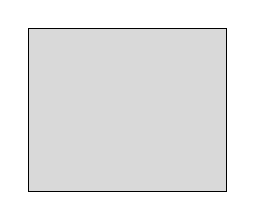
\begin{tikzpicture}[scale=0.9]
        \draw[fill=gray!30!] (0,0) rectangle (2.8,2.3);
        \end{tikzpicture} 
\end{center}
        
        Périmètre = \hrulefill
        
    \task 

    \begin{center}
        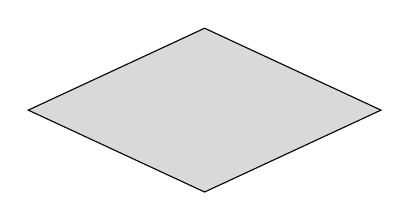
\begin{tikzpicture}[scale=0.8]
        \draw[fill=gray!30!] (0,0) -- (2.8,-1.3) -- (5.6,0) -- (2.8,1.3) -- cycle ;
        \end{tikzpicture} 
\end{center}
        
        Périmètre = \hrulefill
        
    \task 

    \begin{center}
        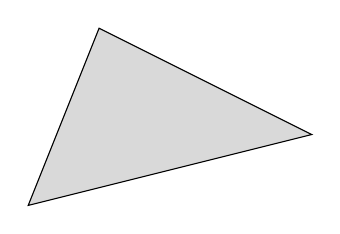
\begin{tikzpicture}[scale=0.9]
        \draw[fill=gray!30!] (0,0) -- (4,1) -- (1,2.5) -- cycle;
        \end{tikzpicture} 
\end{center}
        
        Périmètre = \hrulefill
        
    \task 

    \begin{center}
        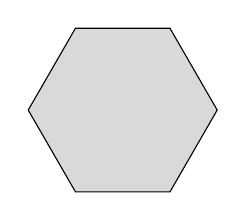
\begin{tikzpicture}[scale=1.2]
        \draw[fill=gray!30!]  (0,0) -- (1,0)-- ++(60:1) -- ++(120:1) -- ++(180:1) -- ++(240:1) -- ++(300:1) -- cycle;
        \end{tikzpicture} 
\end{center}
        
        Périmètre = \hrulefill
    
    \task

    \begin{center}
        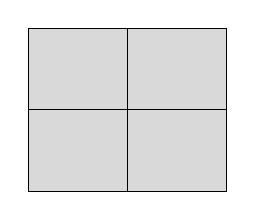
\begin{tikzpicture}[scale=0.9]
        \draw[fill=gray!30!] (0,0) rectangle (2.8,2.3);
        \draw[] (1.4,0) -- (1.4,2.3) ;
        \draw[] (0,1.15) -- (2.8,1.15) ;
        \end{tikzpicture}
\end{center}
        
        Périmètre = \hrulefill
        
    \task 

    \begin{center}
        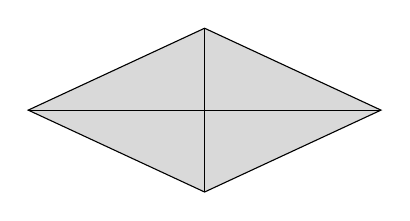
\begin{tikzpicture}[scale=0.8]
        \draw[fill=gray!30!] (0,0) -- (2.8,-1.3) -- (5.6,0) -- (2.8,1.3) -- cycle ;
        \draw[] (0,0) -- (5.6,0) ;
        \draw[] (2.8,-1.3) -- (2.8,1.3) ;
        \end{tikzpicture}
\end{center}
        
        Périmètre = \hrulefill
        
    \task 

    \begin{center}
        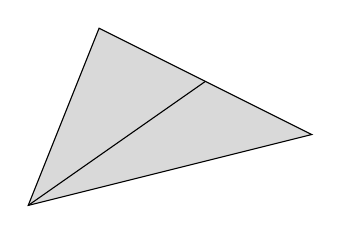
\begin{tikzpicture}[scale=0.9]
        \draw[fill=gray!30!] (0,0) -- (4,1) -- (1,2.5) -- cycle;
        \draw[] (0,0) -- (2.5,1.75);
        \end{tikzpicture}
\end{center}
        
        Périmètre = \hrulefill
        
    \task

    \begin{center}
        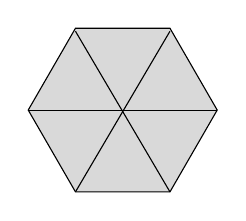
\begin{tikzpicture}[scale=1.2]
        \draw[fill=gray!30!]  (0,0) -- (1,0)-- ++(60:1) -- ++(120:1) -- ++(180:1) -- ++(240:1) -- ++(300:1) -- cycle;
        \draw[] (0,0) -- (1,1.7);
        \draw[] (1,0) -- (0,1.7);
        \draw[] (-0.5,0.86) -- (1.5,0.86);
        \end{tikzpicture} 
\end{center}
        
        Périmètre = \hrulefill
\end{tasks}
\vspace{-0.3cm}
}{1}
\end{exop}


\begin{exop}{
À l'aide de ta règle, prends les mesures nécessaires pour calculer le périmètre des polygones grisés.
\begin{tasks}(2)
    \task 

    \begin{center}
        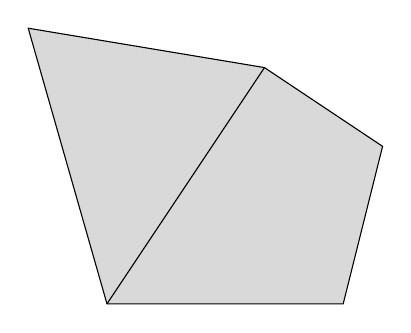
\begin{tikzpicture}
        \draw[fill=gray!30!] (0,0) -- (3,0) -- (3.5,2) -- (2,3) -- (-1,3.5) -- cycle;
        \draw[] (0,0) -- (2,3) ;
        \end{tikzpicture} 
\end{center}
        
        Périmètre = \hrulefill
    
    \task 

    \begin{center}
        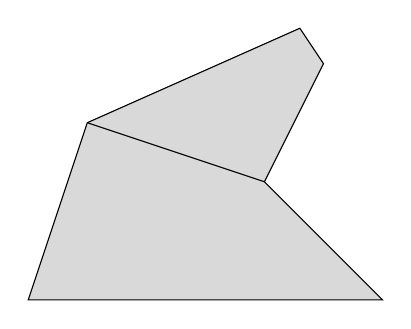
\begin{tikzpicture}[scale=1.5]
        \draw[fill=gray!30!] (0,0) -- (3,0) -- (2,1) -- (2.5,2) -- (2.3,2.3) -- (0.5,1.5) -- cycle;
        \draw[] (2,1) -- (0.5,1.5) ;
        \end{tikzpicture} 
\end{center}
        
        Périmètre = \hrulefill

    \task 

    \begin{center}
        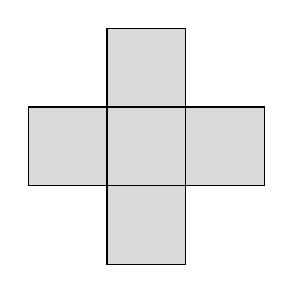
\begin{tikzpicture}
        \draw[fill=gray!30!] (0,0) -- (1,0) -- (1,-1) -- (0,-1) -- (0,-2) -- (-1,-2) -- (-1,-1) -- (-2,-1) -- (-2,0) -- (-1,0) -- (-1,1) -- (0,1) -- cycle;
        \draw[] (0,0) rectangle (-1,-1) ;
        \end{tikzpicture} 
\end{center}
        
        Périmètre = \hrulefill
    
    \task     

    \begin{center}
        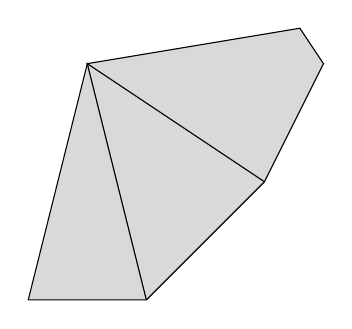
\begin{tikzpicture}[scale=1.5]
        \draw[fill=gray!30!] (0,0) -- (1,0) -- (2,1) -- (2.5,2) -- (2.3,2.3) -- (0.5,2) -- cycle;
        \draw[] (1,0) -- (0.5,2) -- (2,1) ;
        \end{tikzpicture} 
\end{center}
        
        Périmètre = \hrulefill

    \task 

    \begin{center}
        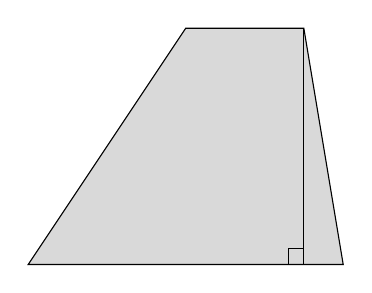
\begin{tikzpicture}
        \draw[fill=gray!30!] (0,0) -- (4,0) -- (3.5,3) -- (2,3) -- (1,1.5) -- cycle;
        \draw (3.5,0) -- (3.5,3) ;
        \draw (3.3,0) -- (3.3,0.2) -- (3.5,0.2) ;
        \end{tikzpicture} 
\end{center}
        
        Périmètre = \hrulefill
    
    \task     

    \begin{center}
        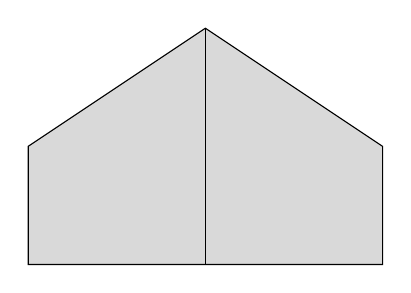
\begin{tikzpicture}[scale=1.5]
        \draw[fill=gray!30!] (0,0) -- (3,0) -- (3,1) -- (1.5,2) -- (0,1) -- cycle ;
        \draw (1.5,2) -- (1.5,0) ;
        \end{tikzpicture} 
\end{center}
        
        Périmètre = \hrulefill
\end{tasks}
}{1}
\end{exop}


\begin{exop}{
Calcule le périmètre des polygones grisés.
\begin{tasks}(2)
    \task 

    \begin{center}
        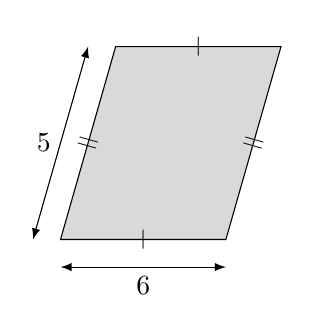
\begin{tikzpicture}[scale=0.7]
        \draw[fill=gray!30] (0,0) -- node[midway, sloped]{{\scriptsize$|$}} (3,0) --node[midway, sloped]{{\scriptsize $||$}} (4,3.5) --node[midway, sloped]{{\scriptsize$|$}} (1,3.5) --node[midway, sloped]{{\scriptsize $||$}} cycle;
        \draw[<->, >=latex] (0,-0.5) --node[midway, below]{$6$} (3,-0.5) ;
        \draw[<->, >=latex] (-0.5,0) --node[midway,left]{$5$} (0.5,3.5);
        \end{tikzpicture} 
\end{center}
        
        Périmètre = \hrulefill
        
    \task 

    \begin{center}
        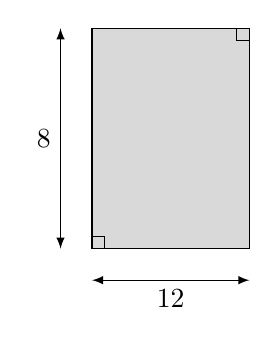
\begin{tikzpicture}[scale=0.8]
        \draw[fill=gray!30] (0,0) rectangle (2.5,3.5);
        \draw (0,0.2) -- (0.2,0.2) -- (0.2,0) ;
        \draw (2.3,3.5) -- (2.3,3.3) -- (2.5,3.3) ;
        \draw[<->, >=latex] (0,-0.5) --node[midway, below]{$12$} (2.5,-0.5) ;
        \draw[<->, >=latex] (-0.5,0) --node[midway, left]{$8$} (-0.5,3.5) ;
        \end{tikzpicture} 
\end{center}
        
        Périmètre = \hrulefill
        
    \task 

    \begin{center}
        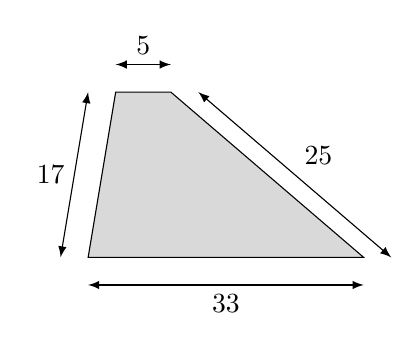
\begin{tikzpicture}[scale=0.7]
        \draw[fill=gray!30] (0,0) -- (5,0) -- (1.5,3) -- (0.5,3) -- cycle ;
        \draw[<->, >=latex] (0,-0.5) --node[midway, below]{$33$} (5,-0.5) ;
        \draw[<->, >=latex] (5.5,0) --node[midway, above right]{$25$} (2,3) ;
        \draw[<->, >=latex] (1.5,3.5) --node[midway, above]{$5$} (0.5,3.5) ;
        \draw[<->, >=latex] (0,3) --node[midway, left]{$17$} (-0.5,0) ;
        \end{tikzpicture} 
\end{center}
        
        Périmètre = \hrulefill
        
    \task     

    \begin{center}
        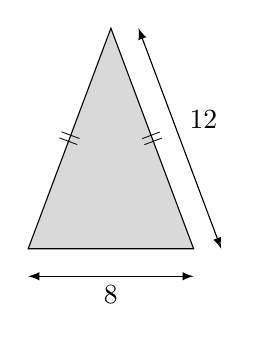
\begin{tikzpicture}[scale=0.7]
        \draw[fill=gray!30] (0,0) -- (3,0) --node[midway, sloped]{{\scriptsize $||$}} (1.5,4) -- node[midway, sloped]{{\scriptsize $||$}}cycle;
        \draw[<->, >=latex] (0,-0.5) --node[midway, below]{$8$} (3,-0.5) ;
        \draw[<->, >=latex] (3.5,0) --node[midway, above right]{$12$} (2,4) ;
        \end{tikzpicture} 
\end{center}
        
        Périmètre = \hrulefill

    \task 

    \begin{center}
        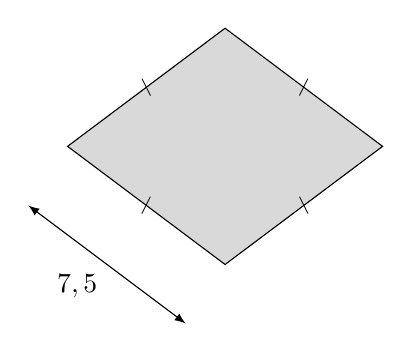
\begin{tikzpicture}[yscale=1.5]
        \draw[fill=gray!30] (-2,0) --node[midway, sloped]{{\scriptsize $|$}} (0,-1) --node[midway, sloped]{{\scriptsize $|$}} (2,0) --node[midway, sloped]{{\scriptsize $|$}} (0,1) --node[midway, sloped]{{\scriptsize $|$}} cycle ;
        \draw[<->, >=latex] (-2.5,-0.5) --node[midway, below left]{$7,5$} (-0.5,-1.5) ;
        \end{tikzpicture} 
\end{center}
        
        Périmètre = \hrulefill
        
    \task     

    \begin{center}
        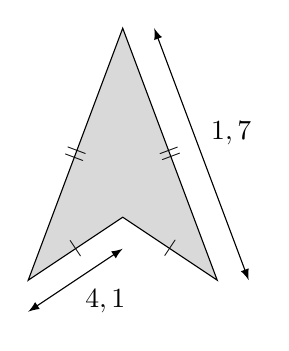
\begin{tikzpicture}[scale=0.8]
        \draw[fill=gray!30] (0,0) --node[midway, sloped]{{\scriptsize $|$}} (1.5,1) --node[midway, sloped]{{\scriptsize $|$}} (3,0) --node[midway, sloped]{{\scriptsize $||$}} (1.5,4) -- node[midway, sloped]{{\scriptsize $||$}}cycle;
        \draw[<->, >=latex] (0,-0.5) --node[midway, below right]{$4,1$} (1.5,0.5) ;
        \draw[<->, >=latex] (3.5,0) --node[midway, above right]{$1,7$} (2,4) ;
        \end{tikzpicture} 
\end{center}
        
        Périmètre = \hrulefill
\end{tasks}
}{1}
\end{exop}

\begin{exol}{GM1}{138}{1}       % P tri, los
\end{exol}


\begin{resolu}{Déterminer une longueur manquante sur un croquis}{
    Plusieurs stratégies peuvent être mises en place pour déterminer une longueur manquante sur un croquis. En voici une liste non exhaustive. 
    \begin{tasks}
        \task Cherche sur le croquis des segments de même longueur.
        
	\begin{center}
        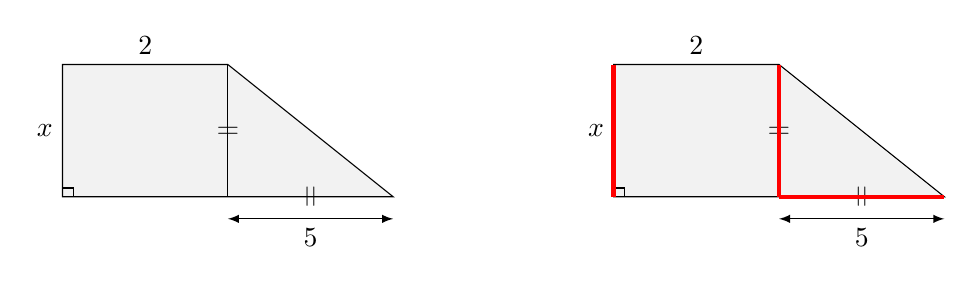
\begin{tikzpicture}[scale=0.7, yscale=0.8]
        \begin{scope}[xshift=-10cm]
            \draw[fill=gray!10] (0,0) -- (3,0) --node[sloped]{{\scriptsize $||$}} (6,0) -- (3,3) --node[above]{$2$} (0,3) --node[left]{$x$} cycle ;
            \draw (0,0.2) -- (0.2,0.2) -- (0.2,0) ;
            \draw[<->, >=latex] (3,-0.5) --node[below]{$5$} (6,-0.5) ;
            \draw[] (3,3) --node[sloped]{{\scriptsize $||$}} (3,0) ;
        \end{scope}
            \draw[fill=gray!10] (0,0) -- (3,0) --node[sloped]{{\scriptsize $||$}} (6,0) -- (3,3) --node[above]{$2$} (0,3) --node[left]{$x$} cycle ;
            \draw (0,0.2) -- (0.2,0.2) -- (0.2,0) ;
            \draw[<->, >=latex] (3,-0.5) --node[below]{$5$} (6,-0.5) ;
            \draw[] (3,3) --node[sloped]{{\scriptsize $||$}} (3,0) ;
            \draw[ultra thick, color=red] (0,0) -- (0,3) ; 
            \draw[ultra thick, color=red] (3,0) -- (6,0) ;
            \draw[ultra thick, color=red] (3,0) -- (3,3) ; 
        \end{tikzpicture}
\end{center}
        \vspace{-0.8cm}
         {\color{blue} Pour déterminer la longueur $x$ de ce trapèze rectangle, on observe le code qui nous indique que $x=5$.}
         
        \task Cherche sur le croquis des segments parallèles dont on connaît la longueur pour en déduire celle que tu cherches.  
	\begin{center}
        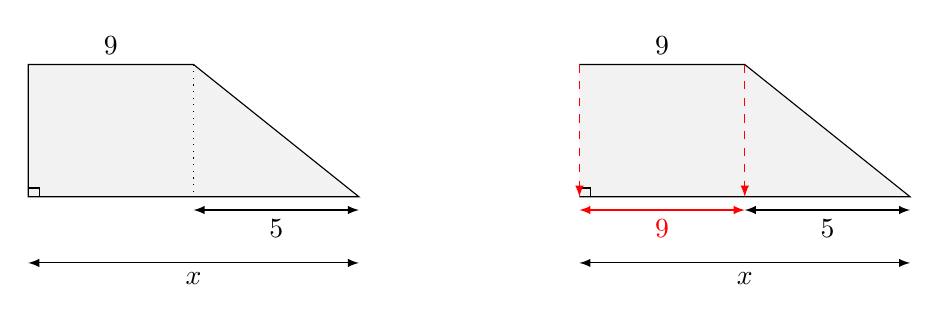
\begin{tikzpicture}[scale=0.7, yscale=0.8]
            \begin{scope}[xshift=-10cm]
                \draw[fill=gray!10] (0,0) -- (3,0) -- (6,0) -- (3,3) --node[above]{$9$} (0,3) -- cycle ;
                \draw (0,0.2) -- (0.2,0.2) -- (0.2,0) ;
                \draw[dotted] (3,3) -- (3,0) ;
                %\draw (3,0.2) -- (3.2,0.2) -- (3.2,0) ;
                \draw[<->, >=latex] (0,-1.5) --node[below]{$x$} (6,-1.5) ;
                \draw[<->, >=latex] (3,-0.3) --node[below] {$5$} (6,-0.3) ;
            \end{scope}
            
            \draw[fill=gray!10] (0,0) -- (3,0) -- (6,0) -- (3,3) --node[above]{$9$} (0,3) ;
            \draw (0,0.2) -- (0.2,0.2) -- (0.2,0) ;
            \draw[->, >=latex, dashed, color=red] (0,3) -- (0,0) ;
            \draw[<->, >=latex] (0,-1.5) --node[below]{$x$} (6,-1.5) ;
            \draw[->, >=latex, dashed, color=red] (3,3) -- (3,0) ;
            \draw[<->, >=latex, color=red] (0,-0.3) --node[below] {$9$} (3,-0.3) ;
            \draw[<->, >=latex] (3,-0.3) --node[below] {$5$} (6,-0.3) ;
        \end{tikzpicture}
\end{center}
\vspace{-0.8cm}
        {\color{blue} Pour déterminer la longueur $x$ de ce trapèze rectangle, on reporte la longueur $9$ sur le segment parallèle et on trouve $x=9+5=14$}
    \end{tasks}
}{1}
\end{resolu}

\newpage 

\begin{exo}{
		Pour chaque polygone, détermine la longueur manquante indiquée par la lettre $x$. Toutes les mesures sont exprimées en $\tunit{}{m}$.
\begin{tasks}(2)
    \task 

    \begin{center}
        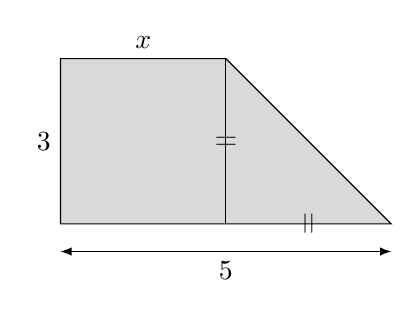
\begin{tikzpicture}[scale=0.7]
            \draw[fill=gray!30] (0,0) -- (3,0) --node[sloped]{{\scriptsize $||$}} (6,0) -- (3,3) --node[above]{$x$} (0,3) --node[left]{$3$} cycle ;
            \draw[<->, >=latex] (0,-0.5) --node[below]{$5$} (6,-0.5) ;
            \draw[] (3,3) --node[sloped]{{\scriptsize $||$}} (3,0) ;
    \end{tikzpicture}
\end{center}
    
    \task 

    \begin{center}
        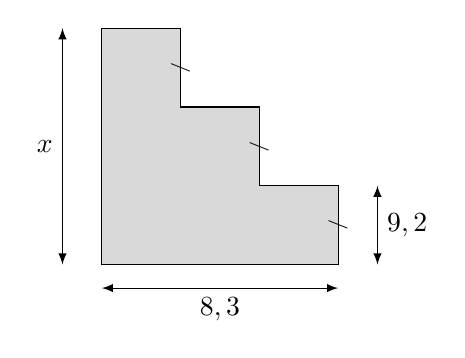
\begin{tikzpicture}
        \draw[fill=gray!30] (1,0) -- (4,0) --node[sloped]{{\scriptsize $/$}} (4,1) -- (3,1) --node[sloped]{{\scriptsize $/$}} (3,2) -- (2,2) --node[sloped]{{\scriptsize $/$}} (2,3) -- (1,3) -- cycle;
        \draw[<->, >=latex] (4.5,0) --node[midway, right]{$9,2$} (4.5,1) ;
        \draw[<->, >=latex] (1,-0.3) --node[midway, below]{$8,3$} (4,-0.3) ;
        \draw[<->, >=latex] (0.5,0) --node[midway, left]{$x$} (0.5,3) ;
\end{tikzpicture}
\end{center}

    \task 

    \begin{center}
        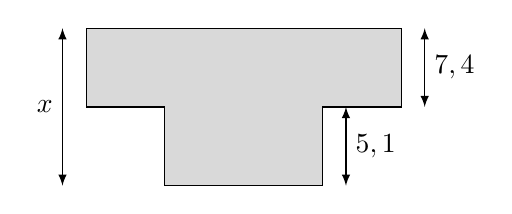
\begin{tikzpicture}[scale=1]
        \draw[fill=gray!30!] (0,0) -- ++(4,0) -- ++(0,-1) -- ++(-1,0) -- ++(0,-1) -- ++(-2,0) -- ++(0,1) -- ++(-1,0) -- ++(0,1) -- cycle ;
        \draw[<->, >=latex] (-0.3,0) --node[midway, left]{$x$} (-0.3,-2) ;
        \draw[<->, >=latex] (3.3,-1) --node[midway, right]{$5,1$} (3.3,-2) ;
        \draw[<->, >=latex] (4.3,0) --node[midway, right]{$7,4$} (4.3,-1) ;
\end{tikzpicture}
\end{center}

    \task 

    \begin{center}
        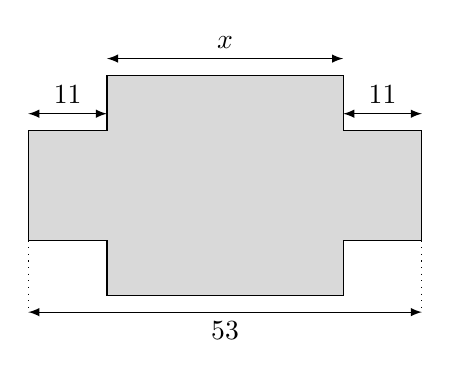
\begin{tikzpicture}[yscale=0.7]
        \draw[fill=gray!30!] (0,0) -- (0,-1) -- (3,-1) -- (3,0) -- (4,0) -- (4,2) -- (3,2) -- (3,3) -- (0,3) -- (0,2) -- (-1,2) -- (-1,0) -- cycle ;
        \draw[dotted] (-1,0) -- (-1,-1.3) ;
        \draw[dotted] (4,0) -- (4,-1.3) ;
        \draw[<->, >=latex] (-1,-1.3) --node[midway, below]{$53$} (4,-1.3) ;
        \draw[<->, >=latex] (0,3.3) --node[midway, above]{$x$} (3,3.3) ;
        \draw[<->, >=latex] (-1,2.3) --node[midway, above]{$11$} (0,2.3) ;
        \draw[<->, >=latex] (3,2.3) --node[midway, above]{$11$} (4,2.3) ;
\end{tikzpicture}
\end{center}

    \task 

    \begin{center}
        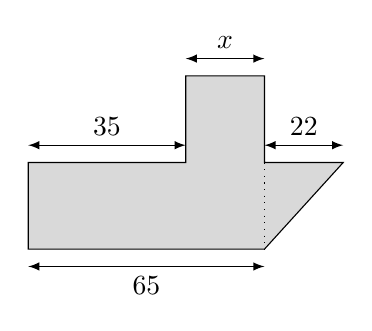
\begin{tikzpicture}[yscale=1.1]
            \draw[fill=gray!30] (0,1) -- (3,1) -- (4,2) -- (3,2) -- (3,3) -- (2,3) -- (2,2) -- (0,2) -- cycle ;
            \draw[<->, >=latex] (0,0.8) --node[midway, below]{$65$} (3,0.8) ;
            \draw[<->, >=latex] (0,2.2) --node[midway, above]{$35$} (2,2.2) ;
            \draw[<->, >=latex] (3,2.2) --node[midway, above]{$22$} (4,2.2) ;
            \draw[<->, >=latex] (2,3.2) --node[midway, above]{$x$} (3,3.2) ;
            \draw[dotted] (3,2) -- (3,1) ;
    \end{tikzpicture}
\end{center}
        
    \task 

    \begin{center}
        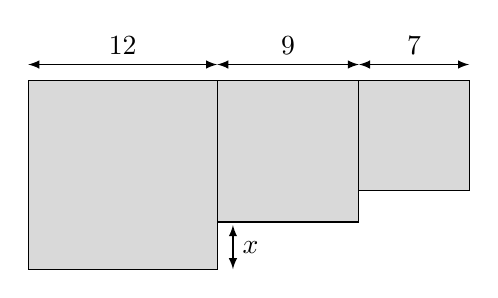
\begin{tikzpicture}[scale=0.4]
        \draw[fill=gray!30] (0,0) rectangle (6,-6) ;
        \draw[fill=gray!30] (6,0) rectangle (10.5,-4.5) ;
        \draw[fill=gray!30] (10.5,0) rectangle (14,-3.5) ;
        \draw[<->, >=latex] (0,.5) --node[midway, above]{$12$} (6,0.5) ;
        \draw[<->, >=latex] (6,.5) --node[midway, above]{$9$} (10.5,0.5) ;
        \draw[<->, >=latex] (10.5,0.5) --node[midway, above]{$7$} (14,0.5) ;

        \draw[<->, >=latex] (6.5,-6) --node[midway, right]{$x$} (6.5,-4.6) ;
\end{tikzpicture}
\end{center}

    
\end{tasks}
}{1}
\end{exo}

\begin{exo}{
Pour chaque polygone, détermine la longueur manquante indiquée par la lettre $x$.
Toutes les mesures sont exprimées en $\tunit{}{cm}$.
\begin{tasks}(2)[after-item-skip = 0.2em]
    \task ~\\
        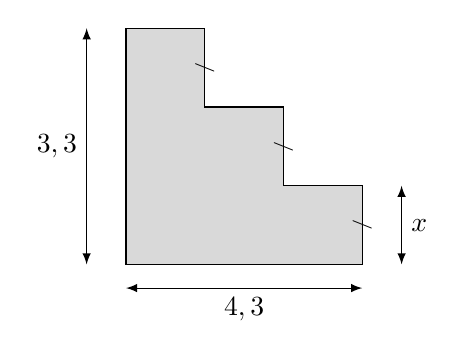
\begin{tikzpicture}
        \draw[fill=gray!30] (1,0) -- (4,0) --node[sloped]{{\scriptsize $/$}} (4,1) -- (3,1) --node[sloped]{{\scriptsize $/$}} (3,2) -- (2,2) --node[sloped]{{\scriptsize $/$}} (2,3) -- (1,3) -- cycle;
        \draw[<->, >=latex] (4.5,0) --node[midway, right]{$x$} (4.5,1) ;
        \draw[<->, >=latex] (1,-0.3) --node[midway, below]{$4,3$} (4,-0.3) ;
        \draw[<->, >=latex] (0.5,0) --node[midway, left]{$3,3$} (0.5,3) ;
        \end{tikzpicture}
	\vspace{-0.5cm}
    \task 

    \begin{center}
        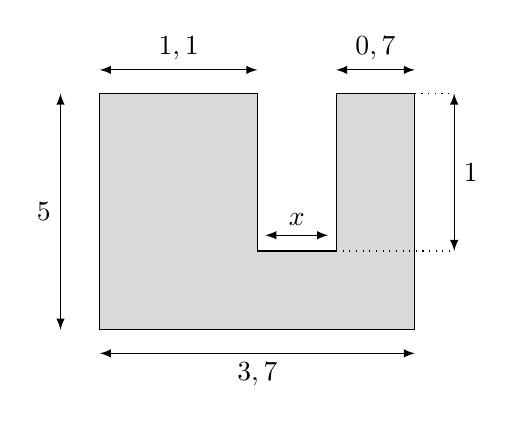
\begin{tikzpicture}[scale=1]
        \draw[fill=gray!30]  (0,0) -- (4,0) -- (4,3) -- (3,3) -- (3,1) -- (2,1) -- (2,3) -- (0,3) -- cycle;
        \draw[<->, >=latex] (2.1,1.2) --node[midway, above]{$x$} (2.9,1.2) ;
        \draw[<->, >=latex] (0,3.3) --node[midway, above]{$1,1$} (2,3.3) ;
        \draw[<->, >=latex] (3,3.3) --node[midway, above]{$0,7$} (4,3.3) ;
        \draw[<->, >=latex] (0,-0.3) --node[midway, below]{$3,7$} (4,-0.3) ;
        \draw[<->, >=latex] (-0.5,0) --node[midway, left]{$5$} (-0.5,3) ;
        \draw[<->, >=latex] (4.5,1) --node[midway, right]{$1$} (4.5,3) ;
        \draw[dotted] (3,1) -- (4.5,1) ;
        \draw[dotted] (4,3) -- (4.5,3) ;
        \end{tikzpicture}
\end{center}
	\vspace{-0.5cm}
    \task 

    \begin{center}
        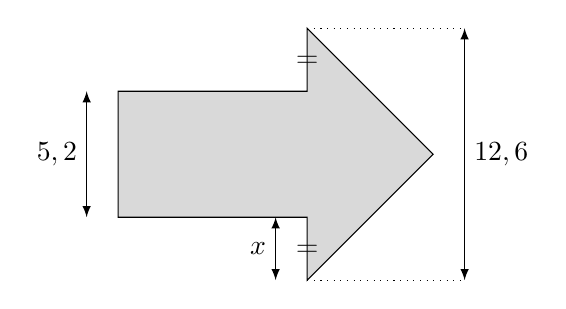
\begin{tikzpicture}[scale=0.8]
            \draw[fill=gray!30] (0,-1) -- (3,-1) --node[sloped]{{\scriptsize $||$}} (3,-2) -- (5,0) -- (3,2) --node[sloped]{ {\scriptsize $||$}} (3,1) -- (0,1) -- cycle ;
            \draw[dotted] (3,2) -- (5.5,2) ;
            \draw[dotted] (3,-2) -- (5.5,-2) ;
            \draw[<->, >=latex] (5.5,-2) --node[midway, right]{$12,6$} (5.5,2) ;
            \draw[<->, >=latex] (-0.5,-1) --node[midway, left]{$5,2$} (-0.5,1) ;
            \draw[<->, >=latex] (2.5,-1) --node[midway, left]{$x$} (2.5,-2) ;
        \end{tikzpicture}
\end{center}
\vspace{-0.5cm}
    \task 

    \begin{center}
        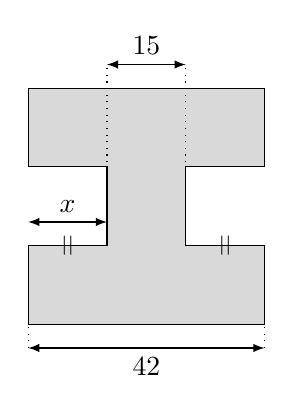
\begin{tikzpicture}
        \draw[fill=gray!30] (0.5,0) -- (3.5,0) -- (3.5,1) --node[sloped]{{\scriptsize $||$}} (2.5,1) -- (2.5,2) -- (3.5,2) -- (3.5,3) -- (0.5,3) -- (0.5,2) -- (1.5,2) -- (1.5,1) --node[sloped]{{\scriptsize $||$}} (0.5,1) -- cycle ;
            \draw[dotted] (3.5,-0.3) -- (3.5,0) ;
            \draw[dotted] (0.5,-0.3) -- (0.5,-0) ;
            \draw[<->, >=latex] (0.5,-0.3) --node[midway, below]{$42$} (3.5,-0.3) ;
            \draw[dotted] (1.5,1.3) -- (1.5,3.3) ;
            \draw[dotted] (2.5,1.3) -- (2.5,3.3) ;
            \draw[<->, >=latex] (1.5,3.3) --node[midway, above]{$15$} (2.5,3.3) ;
            \draw[<->, >=latex] (0.5,1.3) --node[midway, above]{$x$} (1.5,1.3) ;
        \end{tikzpicture}
\end{center}
	\vspace{-0.5cm}
    \task 

    \begin{center}
        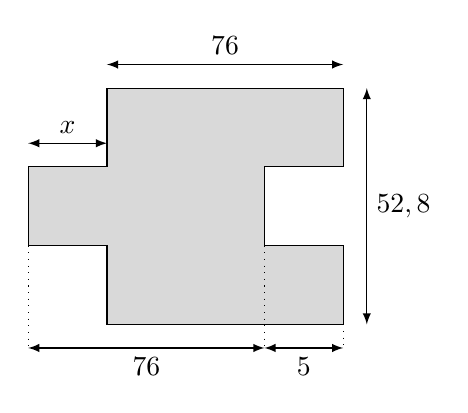
\begin{tikzpicture}
            \draw[fill=gray!30] (1,0) -- (4,0) -- (4,1) -- (3,1) -- (3,2) -- (4,2) -- (4,3) -- (1,3) -- (1,2) -- (0,2) -- (0,1) -- (1,1) -- cycle ;
            %\draw[dotted] (4.3,3) -- (1,3) ;
            %\draw[dotted] (4.3,0) -- (1,0) ;
            \draw[<->, >=latex] (4.3,0) --node[midway, right]{$52,8$} (4.3,3) ;
            
            \draw[dotted] (0,1) -- (0,-0.3) ;
            \draw[dotted] (3,1) -- (3,-0.3) ;
            \draw[<->, >=latex] (0,-0.3) --node[midway, below]{$76$} (3,-0.3);
            \draw[dotted] (4,0) -- (4,-0.3) ;
            \draw[<->, >=latex] (3,-0.3) --node[midway, below]{$5$} (4,-0.3);
            \draw[<->, >=latex] (1,3.3) --node[midway, above]{$76$} (4,3.3);
            \draw[<->, >=latex] (0,2.3) --node[midway, above]{$x$} (1,2.3);
        \end{tikzpicture}
\end{center}
	\vspace{-0.5cm}
        \task 

    \begin{center}
        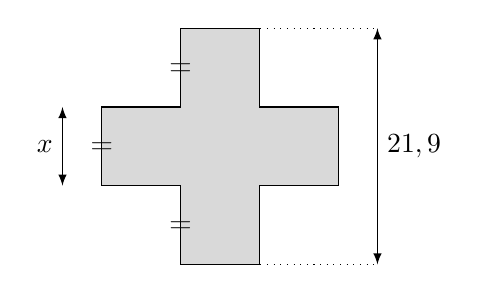
\begin{tikzpicture}
        \draw[fill=gray!30!] (0,0) -- (1,0) -- (1,-1) -- (0,-1) -- (0,-2) -- (-1,-2) --node[sloped]{{\scriptsize $||$}} (-1,-1) -- (-2,-1) --node[sloped]{{\scriptsize $||$}} (-2,0) -- (-1,0) --node[sloped]{{\scriptsize $||$}} (-1,1) -- (0,1) -- cycle;
        \draw[dotted] (-1,1) -- (1.5,1) ;
            \draw[dotted] (-1,-2) -- (1.5,-2) ;
            \draw[<->, >=latex] (1.5,-2) --node[midway, right]{$21,9$} (1.5,1) ;
            \draw[<->, >=latex] (-2.5,-1) --node[midway, left]{$x$} (-2.5,0) ;
            %\draw[<->, >=latex] (2.5,-1) --node[midway, left]{$x$} (2.5,-2) ;
        \end{tikzpicture}
\end{center}

\end{tasks}
}{1}
\end{exo}


\begin{exop}{
		Calcule le périmètre des polygones suivants. L'unité est le $\tunit{}{m}$.

%\begin{multicols}{2}
\begin{tasks}
    \task Croquis à l'échelle. Tous les angles de la figure sont des angles droits. \\
    
    \begin{center}
        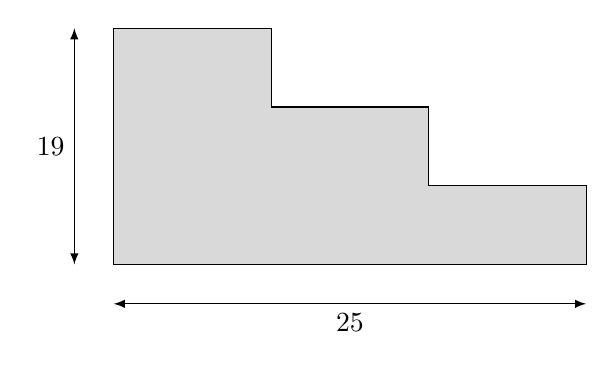
\begin{tikzpicture}
        \draw[fill=gray!30] (0,0) -- (6,0) -- (6,1) -- (4,1) -- (4,2) -- (2,2) -- (2,3) -- (0,3) -- cycle;
        \draw[<->, >=latex] (0,-0.5) --node[midway, below]{$25$} (6,-0.5) ;
        \draw[<->, >=latex] (-0.5,0) --node[midway, left]{$19$} (-0.5,3) ;
        \end{tikzpicture} 
\end{center}
        
        Périmètre = \hrulefill
    \task Croquis à l'échelle. Tous les angles de la figure sont des angles droits.\\
    
    \begin{center}
        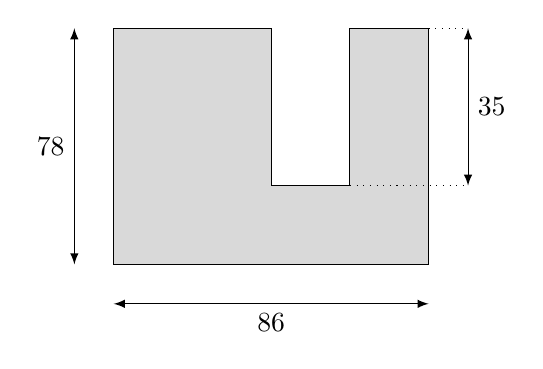
\begin{tikzpicture}[scale=1]
        \draw[fill=gray!30]  (0,0) -- (4,0) -- (4,3) -- (3,3) -- (3,1) -- (2,1) -- (2,3) -- (0,3) -- cycle;
        \draw[<->, >=latex] (0,-0.5) --node[midway, below]{$86$} (4,-0.5) ;
        \draw[<->, >=latex] (-0.5,0) --node[midway, left]{$78$} (-0.5,3) ;
        \draw[<->, >=latex] (4.5,1) --node[midway, right]{$35$} (4.5,3) ;
        \draw[dotted] (3,1) -- (4.5,1) ;
        \draw[dotted] (4,3) -- (4.5,3) ;
        \end{tikzpicture} 
\end{center}
        
        Périmètre = \hrulefill
\end{tasks}
%\end{multicols}
}{1}
\end{exop}


\begin{QSJ}{183}{1}
\end{QSJ}
\begin{exol}{GM5}{138}{1}       % P-A fig-comp rect/carre
\end{exol}
\begin{exof}{GM6}{186}{1}       % mesure plan + convertir échelle
\end{exof}  
\begin{exof}{GM7}{187}{1}       % comparer aires + perim
\end{exof}
\begin{exof}{GM8}{188}{1}       % changement unite aire
\end{exof}
\begin{exof}{GM9}{189}{1}       % changement unite aire
\end{exof}
\begin{exof}{GM10}{189}{1}      % estimer P-A non-polygone
\end{exof}
\begin{exof}{GM12}{190}{1}      % changemnet unite aire et perim
\end{exof}





%----------------------parallélogrammes--------------------



\begin{resolu}{Tracer une hauteur d'un parallélogramme}{Trace la hauteur du parallélogramme correspondant à la paire de bases de ton choix.
%\begin{center} 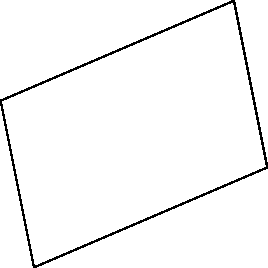
\includegraphics[]{media/gm-01/parallelogramme0.pdf} \end{center}

\begin{tasks}[column-sep=10pt](2)
    \task Choisis une paire de bases. 
    \begin{center} 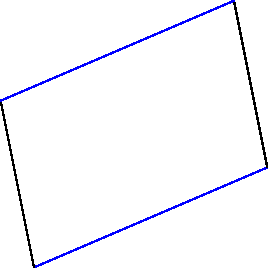
\includegraphics[scale=0.9]{media/gm-01/parallelogramme1} \end{center}

    \task Aligne l'équerre à l'une des bases.
    \begin{center} 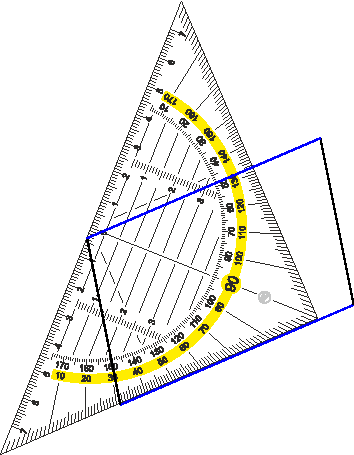
\includegraphics[scale=.9]{media/gm-01/parallelogramme2bis} \end{center}

    \task Dessine une perpendiculaire à la base qui intersecte la base opposée.
    \begin{center} 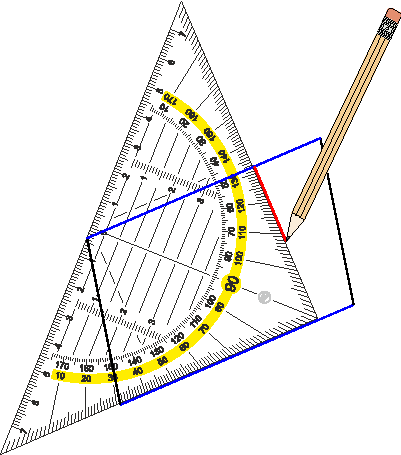
\includegraphics[scale=.9]{media/gm-01/parallelogramme3bis} \end{center}

    \task On obtient :
    \begin{center} 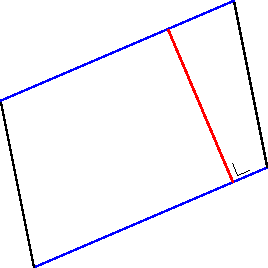
\includegraphics[scale=0.9]{media/gm-01/parallelogramme4}
    \end{center}
\end{tasks}

Parfois, la hauteur du parallélogramme peut se trouver à l'extérieur de la figure. Dans ce cas, prolonge la base autant que nécessaire.
\begin{center} 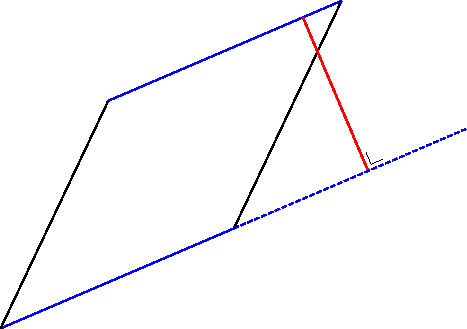
\includegraphics[]{media/gm-01/parallelogramme5}
    \end{center}
}{1}
\end{resolu}


\begin{exol}{GM20}{140}{1}
\end{exol}
\newpage 
\begin{exop}{
Trace les hauteurs des parallélogrammes correspondant aux bases AB.
\begin{tasks}(2)[after-item-skip = 0.2em]
	\task

	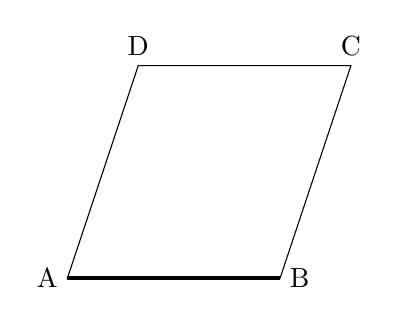
\begin{tikzpicture}[scale=0.9]
        \coordinate (A) at (0,0);
        \coordinate (B) at (3,0);
        \coordinate (C) at (4,3);
        \coordinate (D) at (1,3);        
        \draw[] (A)  node[left]{$\mathrm{A}$} -- (B) node[right]{$\mathrm{B}$} -- (C) node[above]{$\mathrm{C}$} -- (D) node[above]{$\mathrm{D}$} --cycle ;
        \draw[ultra thick] (A) -- (B) ;
\end{tikzpicture}
\vspace{-0.4cm}
		\task

        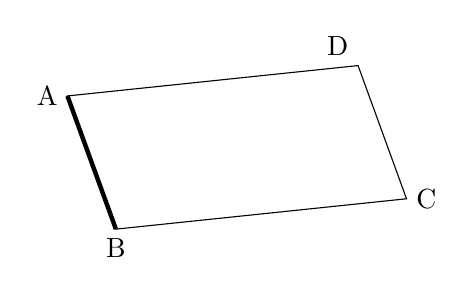
\begin{tikzpicture}[rotate=-70,scale=0.9]
        \coordinate (A) at (0,0);
        \coordinate (B) at (2,0);
        \coordinate (C) at (3,4);
        \coordinate (D) at (1,4);
        \draw[] (A)  node[left]{$\mathrm{A}$} -- (B) node[below ]{$\mathrm{B}$} -- (C) node[right]{$\mathrm{C}$} -- (D) node[above left]{$\mathrm{D}$} --cycle ;
        \draw[ultra thick] (A) -- (B) ;
        \end{tikzpicture}
\vspace{-0.4cm}
\task

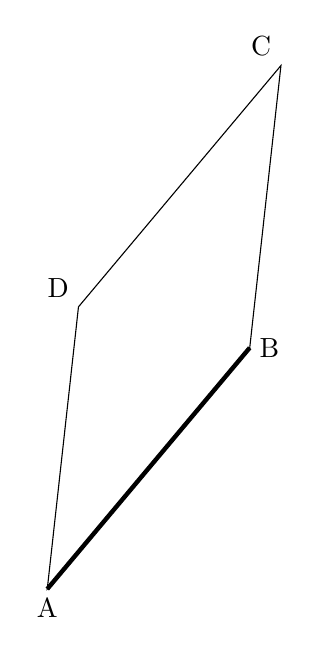
\begin{tikzpicture}[rotate=50]
        \coordinate (A) at (0,0);
        \coordinate (B) at (4,0);
        \coordinate (C) at (7,2);
        \coordinate (D) at (3,2);
        \draw[] (A)  node[below]{$\mathrm{A}$} -- (B) node[right]{$\mathrm{B}$} -- (C) node[above left]{$\mathrm{C}$} -- (D) node[above left]{$\mathrm{D}$} --cycle ;
        \draw[ultra thick] (A) -- (B) ;
        \end{tikzpicture}
\vspace{-0.5cm}
\task

        \begin{tikzpicture}[rotate=0]
        \coordinate (A) at (0,0);
        \coordinate (B) at (2,0);
        \coordinate (C) at (6,4);
        \coordinate (D) at (4,4);
        \draw[] (A)  node[below]{$\mathrm{A}$} -- (B) node[below]{$\mathrm{B}$} -- (C) node[above]{$\mathrm{C}$} -- (D) node[above]{$\mathrm{D}$} --cycle ;
        \draw[ultra thick] (A) -- (B) ;
        \end{tikzpicture}
\vspace{-0.5cm}
	\task

        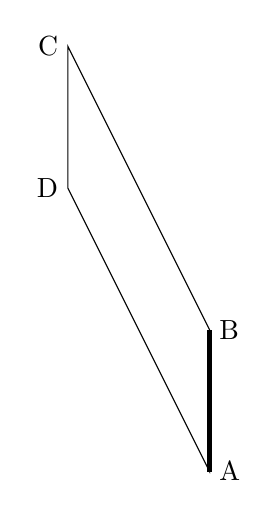
\begin{tikzpicture}[scale=0.9,rotate=90]
        \coordinate (A) at (0,0);
        \coordinate (B) at (2,0);
        \coordinate (C) at (6,2);
        \coordinate (D) at (4,2);
        \draw[] (A)  node[right]{$\mathrm{A}$} -- (B) node[right]{$\mathrm{B}$} -- (C) node[left]{$\mathrm{C}$} -- (D) node[left]{$\mathrm{D}$} --cycle ;
        \draw[ultra thick] (A) -- (B) ;
    \end{tikzpicture}
\vspace{-0.4cm}
\end{tasks}
}{1}
\end{exop}




\begin{exo}{    %parallélogramme
Calcule l'aire d'un parallélogramme qui a :
\begin{tasks}
%\begin{multicols}{2}
	\task $\tunit{3}{dm}$ de base et $\tunit{8}{dm}$ de hauteur correspondante.
	\task $\tunit{4}{km}$ de base et $\tunit{2,5}{km}$ de hauteur correspondante.
	\task $\tunit{1,3}{mm}$ de base et $\tunit{3}{mm}$ de hauteur correspondante.
	\task $\tunit{0,2}{m}$ de base et $\tunit{0,6}{dm}$ de hauteur correspondante.
%\end{multicols}
\end{tasks}
}{1}
\end{exo}




%----------------------triangles----------------------
\begin{exop}{
		Le rectangle ci-dessous a $\tunit{6}{cm}$ de largeur et $\tunit{8}{cm}$ de longueur.\\
\begin{center}
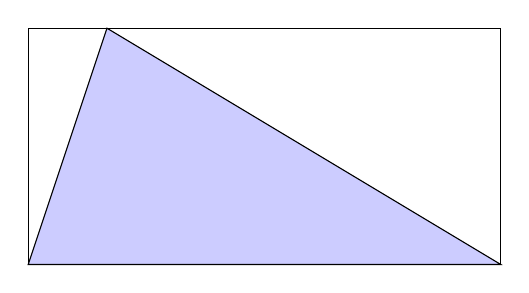
\begin{tikzpicture}
    \draw (0,0) rectangle (6,3) ;
    \draw[fill=blue!20] (0,0) -- (6,0) -- (1,3)  -- cycle ;
\end{tikzpicture}
\end{center}
\begin{tasks}
    \task Calcule l'aire du rectangle. \smallskip \\ \ligne{14.5}
    \task Calcule l'aire du triangle ombré \smallskip \\ \ligne{14.5}
    \task De quelle manière peut-on calculer l'aire d'un triangle ? \smallskip \\ \ligne{14.5}
\end{tasks}
}{1} 
\end{exop}

\begin{exol}{GM21}{140}{1}      %triangle -> parallélogramme
\end{exol}



\begin{exof}{GM25}{192}{1}      %A triangle, papier millimétré (mettre triangle dans une boite)
\end{exof}



\begin{exop}{
Trace les hauteurs des triangles correspondant aux bases AB.
\begin{tasks}[after-item-skip = 0.2em]
    \task ~\\
        \begin{tikzpicture}
        \coordinate (A) at (0,0);
        \coordinate (B) at (3,0);
        \coordinate (C) at (1,3);
        \draw[] (A)  node[left]{$\mathrm{A}$} -- (B) node[right]{$\mathrm{B}$} -- (C) node[above]{$\mathrm{C}$} -- cycle ;
        \draw[ultra thick] (A) -- (B) ;
    
        \begin{scope}[xshift=6cm,rotate=70]
        \coordinate (A) at (0,0);
        \coordinate (B) at (4,0);
        \coordinate (C) at (3,2);
        \draw[] (A)  node[below]{$\mathrm{A}$} -- (B) node[right]{$\mathrm{B}$} -- (C) node[left]{$\mathrm{C}$} -- cycle ;
        \draw[ultra thick] (A) -- (B) ;
        \end{scope}
    
        \begin{scope}[xshift=10cm,yshift=1cm, rotate=-70]
        \coordinate (A) at (0,0);
        \coordinate (B) at (2,0);
        \coordinate (C) at (1,4);
        \draw[] (A)  node[left]{$\mathrm{A}$} -- (B) node[below ]{$\mathrm{B}$} -- (C) node[right]{$\mathrm{C}$} -- cycle ;
        \draw[ultra thick] (A) -- (B) ;
        \end{scope}
        \end{tikzpicture}
        
    \task ~\\
        \begin{tikzpicture}
        \coordinate (A) at (1,0);
        \coordinate (B) at (3,0);
        \coordinate (C) at (-1,3);
        \draw[] (A)  node[left]{$\mathrm{A}$} -- (B) node[right]{$\mathrm{B}$} -- (C) node[above left]{$\mathrm{C}$} -- cycle ;
        \draw[ultra thick] (A) -- (B) ;
    
        \begin{scope}[xshift=8cm,yshift=4cm,rotate=180]
        \coordinate (A) at (0,0);
        \coordinate (B) at (4,0);
        \coordinate (C) at (5,2);
        \draw[] (A)  node[right]{$\mathrm{A}$} -- (B) node[above left]{$\mathrm{B}$} -- (C) node[below left]{$\mathrm{C}$} -- cycle ;
        \draw[ultra thick] (A) -- (B) ;
        \end{scope}
    
        \begin{scope}[xshift=9cm,yshift=2cm, rotate=-70]
        \coordinate (A) at (0,0);
        \coordinate (B) at (2,0);
        \coordinate (C) at (-1,4);
        \draw[] (A)  node[left]{$\mathrm{A}$} -- (B) node[below ]{$\mathrm{B}$} -- (C) node[right]{$\mathrm{C}$} -- cycle ;
        \draw[ultra thick] (A) -- (B) ;
        \end{scope}
        \end{tikzpicture}
        \vspace{5mm}
        
    \task ~\\
        \begin{tikzpicture}[yshift=0cm]
        \coordinate (A) at (0,0);
        \coordinate (B) at (3,0);
        \coordinate (C) at (0,3);
        \draw[] (A)  node[left]{$\mathrm{A}$} -- (B) node[right]{$\mathrm{B}$} -- (C) node[above]{$\mathrm{C}$} -- cycle ;
        \draw[ultra thick] (A) -- (B) ;
    
        \begin{scope}[xshift=6cm,yshift=0cm,rotate=70]
        \coordinate (A) at (0,0);
        \coordinate (B) at (4,0);
        \coordinate (C) at (4,2);
        \draw[] (A)  node[below]{$\mathrm{A}$} -- (B) node[above right]{$\mathrm{B}$} -- (C) node[left]{$\mathrm{C}$} -- cycle ;
        \draw[ultra thick] (A) -- (B) ;
        \end{scope}
    
        \begin{scope}[xshift=13cm,yshift=5cm, rotate=180]
        \coordinate (A) at (0,0);
        \coordinate (B) at (2,0);
        \coordinate (C) at (2,5);
        \draw[] (A)  node[above]{$\mathrm{A}$} -- (B) node[above ]{$\mathrm{B}$} -- (C) node[below]{$\mathrm{C}$} -- cycle ;
        \draw[ultra thick] (A) -- (B) ;
        \end{scope}
        \end{tikzpicture}
\end{tasks}
}{1}
\end{exop}


\begin{resolu}{Calculer l'aire d'un triangle}{
		Calcule l'aire d'un triangle qui a $\tunit{25}{dm}$ de base et $\tunit{1,7}{m}$ de hauteur correspondante.

Démarche :
\vspace{-0.2cm}
\begin{tasks}[after-item-skip = 0.3em]
    \task Vérifie que toutes les longueurs sont exprimées dans la même unité. Si nécessaire, effectue des conversions.
    
{\color{blue} Je convertis mes longueurs en \tunit{}{dm} : $\tunit{1,7}{m}=\tunit{17}{dm}$}
    
    \task Si l'énoncé ne propose pas de croquis, dessine le triangle d'après les indications de l'énoncé.
    \begin{itemize}
        \item Identifie clairement une base et dessine la hauteur correspondante ;
        \item Indique toutes les grandeurs connues.
    \end{itemize}
    \begin{center}
            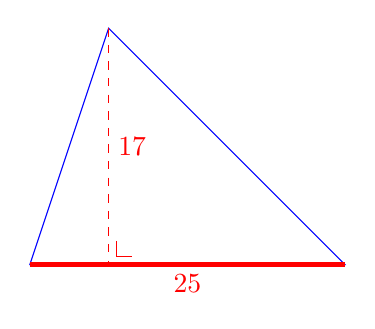
\begin{tikzpicture}[scale=1]
                \draw[color=blue] (0,0) --node[below, color=red]{$25$} (4,0) -- (1,3) -- cycle ;
                \draw[color=red, ultra thick] (0,0) -- (4,0) ;
                \draw[color=red, dashed] (1,3) --node[right] {$17$} (1,0) ;
                \draw[color=red] (1.1,0.3) -- (1.1,0.1) -- (1.3,0.1) ;
            \end{tikzpicture}
    \end{center}
\vspace{-0.8cm}
    \task Utilise la formule d'aire d'un triangle : \fbox{$\textrm{A}_{\textrm{triangle}}=\dfrac{\textrm{base}\cdot\textrm{hauteur}}{2}$}
      
    {\color{blue} $\textrm{A}_{\textrm{triangle}}=\dfrac{25\cdot17}{2}=212,\tunit{5}{dm^2}$
	    \vspace{-0.2cm}
    }
\end{tasks}

}{1}    
\end{resolu}


\begin{exo}{    %triangle
Calcule l'aire d'un triangle qui a :
\vspace{-0.2cm}
\begin{tasks}[after-item-skip = 0.3em]
%\begin{multicols}{2}
	\task $\tunit{15}{mm}$ de base et $\tunit{6}{mm}$ de hauteur correspondante.
	\task $\tunit{0,2}{m}$ de base et $\tunit{0,9}{m}$ de hauteur correspondante.
	\task $\tunit{500}{dm}$ de base et $\tunit{300}{dm}$ de hauteur correspondante.
	\task $\tunit{7}{cm}$ de base et $\tunit{1,1}{cm}$ de hauteur correspondante.
%\end{multicols}
\end{tasks}
\vspace{-0.3cm}
}{1}
\end{exo}

\begin{exo}{    %triangle
Calcule l'aire d'un triangle qui a :
\begin{tasks}[after-item-skip = 0.3em]
%\begin{multicols}{2}
	\task $\tunit{23}{km}$ de base et $\tunit{754}{dam}$ de hauteur correspondante.
	\task $\tunit{16}{m}$ de base et $\tunit{0,9}{hm}$ de hauteur correspondante.
	\task $\tunit{562}{dm}$ de base et $\tunit{300}{dam}$ de hauteur correspondante.
	\task $\tunit{93}{mm}$ de base et $\tunit{1,1}{cm}$ de hauteur correspondante.
%\end{multicols}
\end{tasks}
}{1}
\end{exo}



\begin{exol}{GM26}{141}{1}      %triangles
\end{exol}



\begin{exo}{
Prends les mesures nécessaires pour calculer l'aire des triangles ci-dessous.

\begin{tasks}(2)[after-item-skip = 0.2em]

    \task ~\\    
        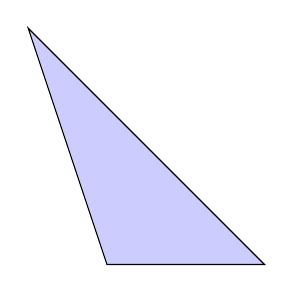
\begin{tikzpicture}
            \draw[fill=blue!20] (0,0) -- (2,0) -- (-1,3) --cycle ;
        \end{tikzpicture}
    \task ~\\    
        \begin{tikzpicture}
            \draw[fill=blue!20] (0,0) -- (3,-1) -- (0,2) --cycle ;
        \end{tikzpicture}
    \task ~\\    
        \begin{tikzpicture}
            \draw[fill=blue!20] (0,0) -- (5,0) -- (2.5,1.5) --cycle ;
        \end{tikzpicture}
    \task ~\\    
        \begin{tikzpicture}
            \draw[fill=blue!20] (0,0) -- (3,0) -- (4,3) --cycle ;
        \end{tikzpicture}
    \task ~\\    
        \begin{tikzpicture}
            \draw[fill=blue!20] (0,0) -- (4,0) -- (-1,2) --cycle ;
        \end{tikzpicture}
    \task ~\\    
        \begin{tikzpicture}
            \draw[fill=blue!20] (0,0) -- (5,0) -- (2,-1.5) --cycle ;
        \end{tikzpicture}
\end{tasks}
}{1}
\end{exo}








%---------------------LOSANGE-----------------

\begin{exop}{
		Le rectangle ci-dessous a $\tunit{9}{cm}$ de largeur et $\tunit{6}{cm}$ de longueur.\\
\begin{center}
\begin{tikzpicture}
    \draw (0,0) rectangle (6,3) ;
    \draw[fill=blue!20] (3,0) -- (6,1.5) -- (3,3) -- (0,1.5) -- cycle ;
\end{tikzpicture}
\end{center}
\begin{tasks}
    \task Calcule l'aire du rectangle. \smallskip \\ \ligne{14.5}
    \task Calcule l'aire du losange ombré \smallskip \\ \ligne{14.5}
    \task De quelle manière peut-on calculer l'aire d'un losange ? \smallskip \\ \ligne{14.5}
\end{tasks}
}{1} 
\end{exop}


\begin{exol}{GM24}{141}{1}      %losange -> rect x3
\end{exol}


\begin{resolu}{Calculer l'aire d'un losange}{
		Calcule l'aire d'un losange dont les diagonales mesures $\tunit{1,7}{m}$ et $\tunit{25}{dm}$.

Démarche :
\begin{tasks}
    \task Vérifie que toutes les longueurs sont exprimées dans la même unité. Si nécessaire, effectue des conversions.
    
    {\color{blue} Je convertis mes longueurs en \tunit{}{dm} : $\tunit{1,7}{m}=17\tunit{17}{dm}$}
    
    \task Si l'énoncé ne propose pas de croquis, dessine le losange d'après les indications de l'énoncé.
    \begin{itemize}
        \item Les diagonales se coupent à angle droit en leur milieu ;
        \item Indique toutes les grandeurs connues.
    \end{itemize}
    \begin{center}
            \begin{tikzpicture}[scale=0.7]
                \draw[color=blue] (-3,0) -- (0,-2) -- (3,0) -- (0,2) -- cycle ;
                \draw[dashed,color=blue] (-3,0) -- (3,0) ;
                \draw[dashed,color=blue] (0,-2) -- (0,2) ;
                \draw[color=blue] (0.3,0.1) -- (0.1,0.1) -- (0.1,0.3) ;
                \draw[color=blue, <->, >=latex] (-3,-2.5) --node[below]{$25$} (3,-2.5) ;
                \draw[color=blue,dotted] (-3,0) -- (-3,-2.5) ;
                \draw[color=blue,dotted] (3,0) -- (3,-2.5) ;
                \draw[color=blue, <->, >=latex] (3.5,-2) --node[right]{$17$} (3.5,2) ;
                \draw[color=blue,dotted] (0,2) -- (3.5,2) ;
                \draw[color=blue,dotted] (0,-2) -- (3.5,-2) ;
            \end{tikzpicture}
    \end{center}
\vspace{-0.8cm}
    \task Utilise la formule d'aire d'un losange : \\
    
    \fbox{$\textrm{A}_{\textrm{losange}}=\dfrac{\textrm{grande diagonale}\cdot\textrm{petite diagonale}}{2}$} \\
      
    $\textrm{A}_{\textrm{losange}}=\dfrac{25\cdot17}{2}=\tunit{212,5}{dm^2}$
\end{tasks}
}{1}   
\end{resolu}

\begin{exo}{    %losange
Calcule l'aire d'un losange dont les diagonales mesurent :
\begin{tasks}(2)
%\begin{multicols}{2}
	\task $\tunit{9}{cm}$ et $\tunit{7}{cm}$
	\task $\tunit{6}{hm}$ et $\tunit{1,5}{hm}$
	\task $\tunit{1,1}{m}$ et $\tunit{8,2}{m}$
	\task $\tunit{0,7}{hm}$ et $\tunit{4}{hm}$
%\end{multicols}
\end{tasks}
}{1}
\end{exo}

\begin{exo}{    %losange
Calcule l'aire d'un losange dont les diagonales mesurent :
\begin{tasks}(2)
%\begin{multicols}{2}
	\task $\tunit{6}{cm}$ et $\tunit{11}{mm}$
	\task $\tunit{43}{km}$ et $\tunit{187}{dam}$
	\task $\tunit{12,9}{m}$ et $\tunit{23}{cm}$
	\task $\tunit{0,5}{dam}$ et $\tunit{300}{dm}$
%\end{multicols}
\end{tasks}
}{1}
\end{exo}





%-----------------------TRAPEZES---------------------



\begin{exol}{GM22}{140}{1}      %trapèze -> parallélogramme
\end{exol}
\begin{exol}{GM23}{140}{1}      %trapèze -> rect
\end{exol}

\begin{resolu}{Trace une hauteur d'un trapèze}{Trace la hauteur du trapèze.
\begin{tasks}[column-sep=10pt](2)
    \task Repère la paire de bases du trapèze.
    \begin{center} 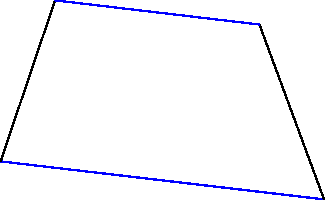
\includegraphics[scale=0.9]{media/gm-01/trapeze1} \end{center}
    \task Aligne l'équerre sur l'une de ses bases.
    \begin{center} 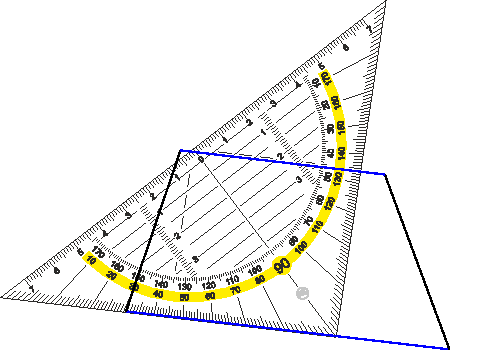
\includegraphics[scale=0.9]{media/gm-01/trapeze2bis} \end{center}
    \task Dessine une perpendiculaire à la base qui intersecte la base opposée.
    \begin{center} 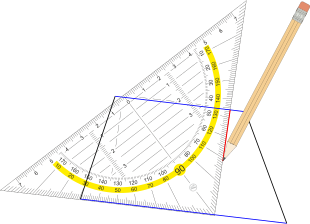
\includegraphics[scale=0.9]{media/gm-01/trapeze3bis} \end{center}
    \task On obtient :
    \begin{center} 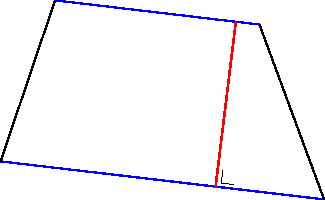
\includegraphics[scale=0.9]{media/gm-01/trapeze4} \end{center}
\end{tasks}

Parfois, la hauteur du trapèze peut se trouver à l'extérieur de la figure. Dans ce cas, prolonge la base autant que nécessaire.
\begin{center} 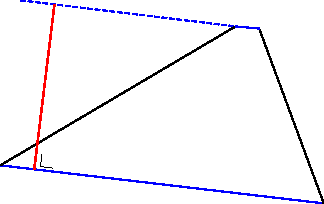
\includegraphics[]{media/gm-01/trapeze5} \end{center}

}{1}
\end{resolu}

\begin{exop}{
Trace les hauteurs des trapèzes correspondant aux bases AB.

\begin{tasks}[after-item-skip = 0.2em]
    \task ~\\
        \begin{tikzpicture}
        \begin{scope}[xshift=0cm,rotate=40]
        \coordinate (A) at (0,0);
        \coordinate (B) at (4,0);
        \coordinate (C) at (3.5,2);
        \coordinate (D) at (2.5,2);
        \draw[] (A)  node[below]{$\mathrm{A}$} -- (B) node[right]{$\mathrm{B}$} -- (C) node[above]{$\mathrm{C}$} -- (D) node[above left]{$\mathrm{D}$} --cycle ;
        \draw[ultra thick] (A) -- (B) ;
        \end{scope}
    
        \begin{scope}[xshift=6cm,yshift=0cm, rotate=0]
        \coordinate (A) at (0,0);
        \coordinate (B) at (2,0);
        \coordinate (C) at (3,4);
        \coordinate (D) at (-1,4);
        \draw[] (A)  node[below]{$\mathrm{A}$} -- (B) node[below ]{$\mathrm{B}$} -- (C) node[above]{$\mathrm{C}$} -- (D) node[above]{$\mathrm{D}$} --cycle ;
        \draw[ultra thick] (A) -- (B) ;
        \end{scope}

        \begin{scope}[xshift=13cm,yshift=0cm, rotate=90]
        \coordinate (A) at (0,0);
        \coordinate (B) at (6,0);
        \coordinate (C) at (5,1);
        \coordinate (D) at (3,1);
        \draw[] (A)  node[below right]{$\mathrm{A}$} -- (B) node[above right]{$\mathrm{B}$} -- (C) node[left]{$\mathrm{C}$} -- (D) node[left]{$\mathrm{D}$} --cycle ;
        \draw[ultra thick] (A) -- (B) ;
        \end{scope}
        \end{tikzpicture}
\vspace{-0.3cm} 
    \task ~\\
        \begin{tikzpicture}
        \begin{scope}[xshift=0cm,rotate=0]
        \coordinate (A) at (0,0);
        \coordinate (B) at (2,0);
        \coordinate (C) at (5,2);
        \coordinate (D) at (2.5,2);
        \draw[] (A)  node[below]{$\mathrm{A}$} -- (B) node[below]{$\mathrm{B}$} -- (C) node[above]{$\mathrm{C}$} -- (D) node[above left]{$\mathrm{D}$} --cycle ;
        \draw[ultra thick] (A) -- (B) ;
        \end{scope}
    
        \begin{scope}[xshift=10cm, yshift=1cm, rotate=180]
        \coordinate (A) at (0,0);
        \coordinate (B) at (1,0);
        \coordinate (C) at (5,3);
        \coordinate (D) at (3,3);
        \draw[] (A)  node[above]{$\mathrm{A}$} -- (B) node[above]{$\mathrm{B}$} -- (C) node[below]{$\mathrm{C}$} -- (D) node[below]{$\mathrm{D}$} --cycle ;
        \draw[ultra thick] (A) -- (B) ;
        \end{scope}
             \begin{scope}[xshift=11cm,yshift=1cm, rotate=-70]
        \coordinate (A) at (0,0);
        \coordinate (B) at (2,0);
        \coordinate (C) at (3,2);
        \coordinate (D) at (0,2);
        \draw[] (A)  node[left]{$\mathrm{A}$} -- (B) node[below ]{$\mathrm{B}$} -- (C) node[right]{$\mathrm{C}$} -- (D)node[above]{$\mathrm{D}$}-- cycle ;
        \draw[ultra thick] (A) -- (B) ;
        \end{scope}
        \end{tikzpicture}
        \vspace{-0.3cm} 
    \task ~\\
        \begin{tikzpicture}
        \coordinate (A) at (0,0);
        \coordinate (B) at (3,0);
        \coordinate (C) at (3,3);
        \coordinate (D) at (-1,3);
        \draw[] (A)  node[left]{$\mathrm{A}$} -- (B) node[right]{$\mathrm{B}$} -- (C) node[above]{$\mathrm{C}$} -- (D)node[above]{$\mathrm{D}$} --cycle ;
        \draw[ultra thick] (A) -- (B) ;
    
        \begin{scope}[xshift=7cm,yshift=2cm,rotate=70]
        \coordinate (A) at (0,0);
        \coordinate (B) at (4,0);
        \coordinate (C) at (4,2);
        \coordinate (D) at (-1,2);
        \draw[] (A)  node[below]{$\mathrm{A}$} -- (B) node[above right]{$\mathrm{B}$} -- (C) node[left]{$\mathrm{C}$} -- (D)node[left]{$\mathrm{D}$}-- cycle ;
        \draw[ultra thick] (A) -- (B) ;
        \end{scope}
       \begin{scope}[xshift=14cm, yshift=-2cm, rotate=100]
        \coordinate (A) at (0,0);
        \coordinate (B) at (4,0);
        \coordinate (C) at (7,1);
        \coordinate (D) at (5,1);
        \draw[] (A)  node[below]{$\mathrm{A}$} -- (B) node[right]{$\mathrm{B}$} -- (C) node[above]{$\mathrm{C}$} -- (D) node[left]{$\mathrm{D}$} --cycle ;
        \draw[ultra thick] (A) -- (B) ;

        \end{scope}


        \end{tikzpicture}
\end{tasks}
\vspace{-0.3cm}
}{1}
\end{exop}




\begin{resolu}{Calculer l'aire d'un trapèze}{
		Calcule l'aire d'un trapèze qui a $\tunit{430}{cm}$ de grande base, $\tunit{17}{dm}$ de petite base et $\tunit{3}{m}$ de hauteur.

Démarche :
\begin{tasks}
    \task Vérifie que toutes les longueurs sont exprimées dans la même unité. Si nécessaire, effectue des conversions.
    
    {\color{blue} Je convertis mes longueurs en \tunit{}{dm} : $\tunit{430}{cm}=\tunit{43}{dm}$ et $\tunit{3}{m}=\tunit{30}{dm}$}
\end{tasks}
\begin{tasks}
	\task[b)] Si l'énoncé ne propose pas de croquis, dessine le losange d'après les indications de l'énoncé.
    \begin{itemize}
        \item Identifie clairement les bases et dessine la hauteur correspondante ;
        \item Indique toutes les grandeurs connues.
    \end{itemize}
\end{tasks}
    \begin{center}
            \begin{tikzpicture}[scale=1]
                \draw[color=blue] (0,0) -- (5,0) -- (3,2) -- (1,2) -- cycle ;
                \draw[dashed,color=red] (1.5,0) --node[right]{$30$} (1.5,2) ;
                \draw[color=red] (1.8,0.1) -- (1.6,0.1) -- (1.6,0.3) ;
                \draw[color=red, ultra thick] (0,0) --node[below]{$43$} (5,0) ;
                \draw[color=red, ultra thick] (3,2) --node[above]{$17$} (1,2) ;
                %\draw[color=blue, <->, >=latex] (-3,-2.5) --node[below]{$25\un{dm}$} (3,-2.5) ;
                %\draw[color=blue,dotted] (-3,0) -- (-3,-2.5) ;
                %\draw[color=blue,dotted] (3,0) -- (3,-2.5) ;
                %\draw[color=blue, <->, >=latex] (3.5,-2) --node[right]{$17\un{dm}$} (3.5,2) ;
                %\draw[color=blue,dotted] (0,2) -- (3.5,2) ;
                %\draw[color=blue,dotted] (0,-2) -- (3.5,-2) ;
            \end{tikzpicture}
    \end{center}
\vspace{-0.8cm}
\begin{tasks}
\task[c)] Utilise la formule d'aire d'un trapèze : \\
    
    \fbox{$\textrm{A}_{\textrm{trapèze}}=\dfrac{\textrm{grande base}\cdot\textrm{petite base}}{2}\cdot\textrm{hauteur}$} \\
      
    $\textrm{A}_{\textrm{trapèze}}=\dfrac{43+17}{2}\cdot30=\dfrac{60}{2}\cdot30=30\cdot30=\tunit{900}{dm^2}$
\end{tasks}
}{1} 
\end{resolu}

\begin{exo}{    %trapèze
Calcule l'aire d'un trapèze qui a :
\begin{tasks}
%\begin{multicols}{2}
	\task $\tunit{25}{dm}$ de grande base, $\tunit{15}{dm}$ de petite base et $\tunit{20}{dm}$ de hauteur.
	\task $\tunit{8}{m}$ de grande base, $\tunit{6}{m}$ de petite base et $\tunit{9}{m}$ de hauteur
	\task $\tunit{60}{mm}$ de grande base, $\tunit{70}{mm}$ de petite base et $\tunit{80}{mm}$ de hauteur
	\task $\tunit{7}{dam}$ de grande base, $\tunit{3}{dam}$ de petite base et $\tunit{80}{m}$ de hauteur
%\end{multicols}
\end{tasks}
}{1}
\end{exo}

\begin{exo}{    %trapèze
Calcule l'aire d'un trapèze qui a :
\begin{tasks}
%\begin{multicols}{2}
	\task $\tunit{0,14}{dam}$ de grande base, $\tunit{26}{m}$ de petite base et $\tunit{10}{dm}$ de hauteur.
	\task $\tunit{900}{cm}$ de grande base, $\tunit{5}{m}$ de petite base et $\tunit{4,5}{dam}$ de hauteur
	\task $\tunit{5,9}{km}$ de grande base, $\tunit{0,8}{km}$ de petite base et $\tunit{40}{dam}$ de hauteur
	\task $\tunit{6}{hm}$ de grande base, $\tunit{1,04}{km}$ de petite base et $\tunit{80}{m}$ de hauteur
%\end{multicols}
\end{tasks}
}{1}
\end{exo}







%-------------------POLYGONES SIMPLES----------------



\begin{exo}{ %mix
\begin{tasks}[after-item-skip = 0.3em]
%\begin{multicols}{2}
	\task Calcule l'aire d'un parallélogramme qui a $\tunit{13}{cm}$ de base et $\tunit{5}{dm}$ de hauteur correspondante.
	\task Calcule l'aire d'un triangle qui a $\tunit{25}{mm}$ de base et $\tunit{3}{dm}$ de hauteur correspondante.
	\task  Calcule l'aire d'un losange dont les diagonales mesurent $\tunit{1,5}{km}$ et $\tunit{7}{dam}$.
	\task Calcule l'aire d'un trapèze qui a $\tunit{17}{m}$ de grande base, $\tunit{2,3}{dam}$ de petite base et $\tunit{780}{cm}$ de hauteur.
%\end{multicols}
\end{tasks}
\vspace{-0.3cm}
}{1}    
\end{exo}


\begin{exo}{
Prends les mesures nécessaires pour calculer l'aire des quadrilatères ci-dessous.
\vspace{-0.3cm}
\begin{tasks}(1)
    \task  %parallélogrammes

    \begin{tikzpicture}[scale=0.8]
        \coordinate (A) at (0,0);
        \coordinate (B) at (3,0);
        \coordinate (C) at (4,3);
        \coordinate (D) at (1,3);        
        \draw[] (A) -- (B) -- (C) -- (D) --cycle ;
    
        \begin{scope}[xshift=6cm,yshift=-2cm,rotate=30]
        \coordinate (A) at (0,0);
        \coordinate (B) at (4,0);
        \coordinate (C) at (7,2);
        \coordinate (D) at (3,2);
        \draw[] (A) -- (B) -- (C) -- (D) --cycle ;
        \end{scope}
    
        \begin{scope}[xshift=12cm,yshift=2cm, rotate=-70]
        \coordinate (A) at (0,0);
        \coordinate (B) at (2,0);
        \coordinate (C) at (3,4);
        \coordinate (D) at (1,4);
        \draw[] (A) -- (B) -- (C) -- (D) --cycle ;
        \end{scope}
    \end{tikzpicture}

    \task

        \begin{tikzpicture}[scale=0.8]
        \begin{scope}[xshift=0cm,yshift=0cm,rotate=70]
        \coordinate (A) at (0,0);
        \coordinate (B) at (4,0);
        \coordinate (C) at (4,2);
        \coordinate (D) at (-1,2);
        \draw[] (A)   -- (B) -- (C) -- (D)-- cycle ;
        \end{scope}
        
        \begin{scope}[xshift=5cm,yshift=0cm,rotate=40]
        \coordinate (A) at (0,0);
        \coordinate (B) at (4,0);
        \coordinate (C) at (3.5,2);
        \coordinate (D) at (2.5,2);
        \draw[] (A)   -- (B)  -- (C)  -- (D)  --cycle ;
        \end{scope}

        \begin{scope}[xshift=13cm,yshift=0cm, rotate=90]
        \coordinate (A) at (0,0);
        \coordinate (B) at (6,0);
        \coordinate (C) at (5,2);
        \coordinate (D) at (3,2);
        \draw[] (A)  -- (B) -- (C) -- (D) --cycle ;
        \end{scope}
        \end{tikzpicture}
        
    \task

        \begin{tikzpicture}[scale=0.9]
        \begin{scope}[xshift=0cm,rotate=40]
        \coordinate (A) at (0,0);
        \coordinate (B) at (2,-1);
        \coordinate (C) at (4,0);
        \coordinate (D) at (2,1);
        \draw[] (A)   -- (B)  -- (C)  -- (D)  --cycle ;
        \end{scope}
    
        \begin{scope}[xshift=6cm,yshift=-2cm,rotate=70]
        \coordinate (A) at (0,0);
        \coordinate (B) at (3,-0.8);
        \coordinate (C) at (6,0);
        \coordinate (D) at (3,0.8);
        \draw[] (A)   -- (B) -- (C) -- (D)-- cycle ;
        \end{scope}

        \begin{scope}[xshift=12cm,yshift=0cm, rotate=90]
        \coordinate (A) at (0,0);
        \coordinate (B) at (2,-2);
        \coordinate (C) at (4,0);
        \coordinate (D) at (2,2);
        \draw[] (A)  -- (B) -- (C) -- (D) --cycle ;
        \end{scope}
        \end{tikzpicture}
\end{tasks}
\vspace{-0.3cm}
}{1}
\end{exo}

\begin{exo}{
Prends les mesures nécessaires pour calculer l'aire des quadrilatères ci-dessous.

\begin{tasks}(1)
    \task ~\\ %parallélogramme
    \begin{tikzpicture}
        \begin{scope}[xshift=0cm,yshift=-10cm, rotate=0]
        \coordinate (A) at (0,0);
        \coordinate (B) at (2,0);
        \coordinate (C) at (6,4);
        \coordinate (D) at (4,4);
        \draw[] (A)   -- (B) -- (C)  -- (D)  --cycle ;
        \end{scope}
	
       \begin{scope}[xshift=10cm, yshift=-12cm, rotate=100]
        \coordinate (A) at (0,0);
        \coordinate (B) at (4,0);
        \coordinate (C) at (7,1);
        \coordinate (D) at (5,1);
        \draw[] (A)   -- (B)  -- (C)  -- (D) --cycle ;
        \end{scope}

        \begin{scope}[xshift=14cm,yshift=-12cm, rotate=90]
        \coordinate (A) at (0,0);
        \coordinate (B) at (2,0);
        \coordinate (C) at (6,2);
        \coordinate (D) at (4,2);
        \draw[] (A)  -- (B)  -- (C) -- (D) --cycle ;
        \end{scope}    
    \end{tikzpicture}

    \task ~\\ %trapèzes
        \begin{tikzpicture}
        \begin{scope}[xshift=0cm,rotate=0]
        \coordinate (A) at (0,0);
        \coordinate (B) at (2,0);
        \coordinate (C) at (5,2);
        \coordinate (D) at (2.5,2);
        \draw[] (A)   -- (B) -- (C)  -- (D)  --cycle ;
        \end{scope} 
            
        \begin{scope}[xshift=14cm, yshift=3cm, rotate=180]
        \coordinate (A) at (0,0);
        \coordinate (B) at (1,0);
        \coordinate (C) at (5,3);
        \coordinate (D) at (3,3);
        \draw[] (A) -- (B) -- (C) -- (D) --cycle ;
        \end{scope}
        \end{tikzpicture}
        \vspace{5mm}
\end{tasks}
}{1}
\end{exo}



%lien A-P rectanle
\begin{exol}{GM37}{145}{1}      %maximiser aire avec un perim fixé
\end{exol}
\begin{exol}{GM42}{147}{1}      %echiquier
\end{exol}  

%(comprendre que triangles+parallélogrammes avec meme base et hauteur ont meme aire)
\begin{exol}{GM38}{146}{1}
\end{exol}
\begin{exol}{GM39}{146}{1}
\end{exol}
\begin{exol}{GM43}{147}{2}      %aire du triangle moitie du rectangle (boite)
\end{exol}
\begin{exol}{GM44}{148}{1}      %sensibilisation a la recherche d'inconnue
\end{exol}
\begin{exol}{GM46}{148}{2}      %construire polygone avec triangles rectangles
\end{exol}
\begin{exol}{GM47}{148}{2}      %comparer aire losanges meme base et hauteur
\end{exol}
\begin{exof}{GM45}{196}{1}      % aire parallélogramme egal rectangle
\end{exof}      

\begin{exol}{GM27}{141}{1}      %para-trap-los
\end{exol}
\begin{exof}{GM28}{193}{1}      % mesure P-A et conversion unite
\end{exof}  
\begin{exof}{GM29}{194}{1}      % mesure A
\end{exof} 
\begin{exof}{GM30}{194}{1}      % mesure P-A 
\end{exof}  
\begin{exol}{GM31}{142}{1}      %figure composée (puzzle)
\end{exol}
\begin{FLP}{195}{1}
\end{FLP}




%--------------------figures composées-------------
\newpage
\begin{exo}{
Calcule l'aire et le périmètre des surfaces ci-dessous, après avoir pris les mesures nécessaires.
\begin{tasks}(2)
    \task ~\\
        \begin{tikzpicture}[xscale=0.5]
            \draw[fill=blue!20] (0,0) -- (5,0) -- (5,1) -- (8,1) -- (8,4) -- (2,4) -- (2,5) -- (0,5) -- cycle ; 
        \end{tikzpicture}

    \task ~\\
        \begin{tikzpicture}
            \begin{scope}[rotate=180]
            \draw[fill=blue!20] (-3,-3) rectangle (3,3) ;
            \draw[fill=white] (-2,-2) rectangle (2,2) ;
            \end{scope}
        \end{tikzpicture}

\end{tasks}
}{1}
\end{exo}



\begin{exo}{
		Calcule l'aire et le périmètre des surfaces ci-dessous. Les unités sont exprimées en \tunit{}{m}.
\begin{tasks}(2)
    \task \textit{Tous les angles de la figure sont des angles droits.}\\
        \begin{tikzpicture}
            \begin{scope}[yscale=1.3,rotate=0]
            \draw[fill=blue!20] (0,0) -- (5,0) -- (5,2) -- (3,2) -- (3,3) -- (1,3) -- (1,4) -- (0,4) -- cycle ;
            \draw[<->, >=latex] (0,4.5) -- (1,4.5) node[midway, above]{$12$} ;
            \draw[dotted] (0,4.5) -- (0,4) ;
            \draw[dotted] (1,4.5) -- (1,4) ;
            \draw[<->, >=latex] (1,4.5) -- (3,4.5) node[midway, above]{$8$} ;
            \draw[dotted] (3,4.5) -- (3,3) ;
            \draw[<->, >=latex] (3,4.5) -- (5,4.5) node[midway, above]{$7$} ;
            \draw[dotted] (5,4.5) -- (5,2) ;
            \draw[<->, >=latex] (5.5,2) -- (5.5,0) node[midway, above, sloped]{$12$} ;
            \draw[dotted] (5,0) -- (5.5,0) ;
            \draw[dotted] (5,2) -- (5.5,2) ;
            \draw[<->, >=latex] (5.5,3) -- (5.5,2) node[midway, above, sloped]{$8$} ;
            \draw[dotted] (3,3) -- (5.5,3) ;
            \draw[<->, >=latex] (5.5,4) -- (5.5,3) node[midway, above, sloped]{$6$} ;
            \draw[dotted] (1,4) -- (5.5,4) ;
            \end{scope}
        \end{tikzpicture}

    \task \textit{Tous les angles de la figure sont des angles droits.}\\
        \begin{tikzpicture}
            \begin{scope}[xscale=0.9,rotate=0]
            \draw[fill=blue!20] (0,0) -- (1,0) -- (1,1) -- (4,1) -- (4,3) -- (3,3) -- (3,5) -- (0,5) -- cycle ;
            \draw[<->, >=latex] (0,-0.5) -- (1,-0.5) node[midway, below]{$4,5$} ;
            \draw[dotted] (0,0) -- (0,-0.5) ;
            \draw[dotted] (1,0) -- (1,-0.5) ;
            \draw[<->, >=latex] (4.5,3) -- (4.5,1) node[midway, above, sloped]{$6,2$} ;
            \draw[dotted] (4.5,1) -- (4,1) ;
            \draw[<->, >=latex] (4.5,5) -- (4.5,3) node[midway, above, sloped]{$4,5$} ;
            \draw[dotted] (4,3) -- (4.5,3) ;
            \draw[dotted] (3,5) -- (4.5,5) ;
            \draw[<->, >=latex] (3,5.5) -- (4,5.5) node[midway, above]{$3,7$} ;
            \draw[dotted] (4,3) -- (4,5.5) ;
            \draw[dotted] (3,5) -- (3,5.5) ;
            \draw[<->, >=latex] (0,5.5) -- (3,5.5) node[midway, above]{$8,5$} ;
            \draw[dotted] (0,5) -- (0,5.5) ;
            \draw[<->, >=latex] (-0.5,0) -- (-0.5,5) node[midway, above, sloped]{$14,1$} ;
            \draw[dotted] (0,5) -- (-0.5,5) ;
            \draw[dotted] (0,0) -- (-0.5,0) ;
            \end{scope}
        \end{tikzpicture}
\end{tasks}
}{1}
\end{exo}

\begin{exo}{
Calcule l'aire de la figure représentée par le croquis ci-dessous. Les proportions et les angles ont été conservés. Les unités sont exprimées en dm.
\begin{center}
    \begin{tikzpicture}[scale=0.6]
    \draw[fill=blue!20] (0,3) -- (1,-5) -- (2,-5) -- (2,-3) -- (4,-1) -- (6,-3) -- (6,-9) -- (0,-9) ;  
    \draw[fill=blue!20] (0,3) -- (-1,-5) -- (-2,-5) -- (-2,-3) -- (-4,-1) -- (-6,-3) -- (-6,-9) -- (0,-9) ;
    \draw[dashed, color=red, ultra thick] (0,4) -- (0,-10) ;
    \node[color=red] at (0,5) {axe de symétrie} ;
    \draw[dotted] (0,3) -- (-6.5,3) ;
    \draw[dotted] (-4,-1) -- (-6.5,-1) ;
    \draw[dotted] (-6,-3) -- (-6.5,-3) ;
    \draw[dotted] (-2,-5) -- (-6.5,-5) ;
    \draw[dotted] (-6,-9) -- (-6.5,-9) ;
    \draw[<->,>=latex] (-6.5,-1) -- (-6.5,3) node[midway, left]{$35$};
    \draw[<->,>=latex] (-6.5,-3) -- (-6.5,-1) node[midway, left]{$10$};
    \draw[<->,>=latex] (-6.5,-5) -- (-6.5,-3) node[midway, left]{$10$};
    \draw[<->,>=latex] (-6.5,-9) -- (-6.5,-5) node[midway, left]{$25$};
    \draw[dotted] (-6,-9) -- (-6,-9.5) ;
    \draw[dotted] (-2,-5) -- (-2,-9.5) ;
    \draw[dotted] (-1,-5) -- (-1,-9.5) ;
    \draw[<->,>=latex] (-6,-9.5) -- (-2,-9.5) node[midway, below]{$20$};
    \draw[<->,>=latex] (-2,-9.5) -- (-1,-9.5) node[midway, below]{$6$};
    \draw[<->,>=latex] (-1,-9.5) -- (0,-9.5) node[midway, below]{$6$};
\end{tikzpicture}
\end{center}
}{2}
\end{exo}


\begin{exol}{GM32}{143}{1}      % P
\end{exol}
\begin{exol}{GM33}{143}{1}      % A-P carrés
\end{exol}
\begin{exol}{GM34}{144}{2}      %A-P simple et comp
\end{exol}
\begin{exol}{GM35}{145}{1}      %A-P croix suisse
\end{exol}
\begin{exol}{GM36}{145}{2}      %A fer lance
\end{exol}
\begin{exol}{GM41}{147}{1}      %divers
\end{exol}
\begin{exol}{GM48}{149}{1}      %terrain a vendre rect+trap A
\end{exol}  
\begin{exol}{GM49}{149}{1}      %terrain foot P-A
\end{exol}
\begin{exol}{GM50}{150}{1}      %sensibilisation recherche côté carré
\end{exol}
\begin{exol}{GM51}{150}{2}
\end{exol}
\begin{exol}{GM52}{151}{2}
\end{exol}
\begin{exol}{GM53}{151}{3}
\end{exol}


\begin{exo}{
		Dans une plaque d'aluminium en forme de parallélogramme, on découpe deux triangles rectangles isocèles. \\ Quel est le poids de la partie restante, sachant que $\tunit{1}{cm^2}$ de cette plaque pèse $\tunit{0,5}{g}$ ? \\
\begin{center}
\begin{tikzpicture}
    \draw[fill=blue!20] (0,0) -- (6,0) -- (8,3) -- (2,3) -- cycle;
    \draw[fill=white] (0,0) -- (3,3) -- (3,0) -- (6,3) -- (6,0) -- cycle ;
    \draw[<->, >=latex] (0,-0.5) --node[midway, below]{$\tunit{24}{cm}$} (6,-0.5) ;
\end{tikzpicture}
\end{center}
}{2}
\end{exo}


\begin{exo}{
    Calcule l'aire de ce panneau indicateur. 
    Toutes les mesures sont exprimées en $\tunit{}{dm}$.
    \begin{center}
        \begin{tikzpicture}
            \draw[fill=blue!20] (0,0) -- (1,1) -- (5,1) -- (4,0) -- (5,-1) -- (1,-1) -- cycle ;
            \node at (2.5,0.2) {\textbf{GENÈVE}} ;
            \node at (2.5,-0.3) {$27\un{km}$} ;

            \draw[<->,>=latex] (-0.2,0.2) --node[midway, above, sloped]{$3,1$} (0.8,1.2) ;
            \draw[<->,>=latex] (-0.2,-0.2) --node[midway, below, sloped]{$3,1$} (0.8,-1.2) ;
            \draw[<->,>=latex] (1,1.3) --node[midway, above]{$12,5$} (5,1.3) ;
            \draw[<->,>=latex] (1,-1.3) --node[midway, below]{$12,5$} (5,-1.3) ;
            \draw[<->,>=latex] (0,-2) --node[midway, below]{$12,5$} (4,-2) ;
            \draw[<->,>=latex] (5.5,-1) --node[midway, right]{$4,2$} (5.5,1) ;
            \draw[dotted] (0,0) -- (0,-2) ;
            \draw[dotted] (4,0) -- (4,-2) ;
        \end{tikzpicture}
    \end{center}
}{2}    
\end{exo}



\begin{exo}{
		\vspace{-0.5cm}
\begin{tasks}[after-item-skip = 0.2em]
    \task On double la longueur et la largeur d'un rectangle. Que devient son périmètre ? Que devient son aire ?
    \task On triple la longueur et la largeur d'un rectangle. Que devient son périmètre ? Que devient son aire ?
    \task On quadruple la longueur et la largeur d'un rectangle. Que devient son périmètre ? Que devient son aire ?
\end{tasks}
}{1}    
\end{exo}



\begin{exo}{
		Un paysan veut échanger un terrain rectangulaire de $\tunit{50}{m}$ sur $\tunit{145}{m}$ contre un champ carré de $\tunit{85}{m}$ de côté. \\ Quelle aire perdra-t-il ?
}{1}    
\end{exo}

\begin{exo}{
		Un jardin rectangulaire de $\tunit{15}{m}$ sur $\tunit{7}{m}$ est traversé, dans le sens de la longueur, par une allée de $\tunit{1,5}{m}$ de large. \\ Fais un croquis de la situation, puis calcule l'aire de la surface cultivable.
}{1}
\end{exo}

\begin{exo}{
		Un carré est inscrit dans un autre carré dont le côté mesure $\tunit{16}{m}$. Calcule l'aire du petit carré.
\begin{center}
    \begin{tikzpicture}
        \draw (0,0) --node[midway, sloped]{{\scriptsize $||$}} (2,0) --node[midway, sloped]{{\scriptsize $||$}} (4,0) --node[midway, sloped]{{\scriptsize $||$}} (4,2) --node[midway, sloped]{{\scriptsize $||$}} (4,4) --node[midway, sloped]{{\scriptsize $||$}} (2,4) --node[midway, sloped]{{\scriptsize $||$}} (0,4) --node[midway, sloped]{{\scriptsize $||$}} (0,2) --node[midway, sloped]{{\scriptsize $||$}} cycle ;
        \draw (2,0) -- (4,2) -- (2,4) -- (0,2) -- cycle;
	\draw[<->, >=latex] (0,-0.5) --node[midway, below]{$\tunit{16}{m}$} (4,-0.5) ;
    \end{tikzpicture}
\end{center}

}{2}    
\end{exo}

\begin{exo}{
$\mathrm{ABCD}$ et $\mathrm{EFGH}$ sont des rectangles. Calcule, dans chaque figure, l'aire de la partie ombrée.
\begin{center}
    \begin{tikzpicture}
\draw (0,0) rectangle (4,2) ;
\draw[fill=blue!20] (0,0) -- (4,1) -- (4,2) -- (2,1) -- (2,2) -- cycle ;
\draw[dotted] (0,1) -- (4,1) ;
\draw[dotted] (2,0) -- (2,2) ;
\node[below left] at (0,0) {$\mathrm{A}$} ;
\node[below right] at (4,0) {$\mathrm{D}$} ;
\node[above left] at (0,2) {$\mathrm{B}$} ;
\node[above right] at (4,2) {$\mathrm{C}$} ;

\draw[<->, >=latex] (0,-0.3) --node[below]{$405\un{m}$} (4,-0.3) ;

\draw[<->, >=latex] (-0.3,0) --node[left]{$135\un{m}$} (-0.3,2) ;


\begin{scope}[xshift=8cm]
\draw (0,0) rectangle (4,2) ;
\draw[fill=blue!20] (0,2) -- (2,0) -- (4,2) -- (2,1) -- cycle ;
\draw[dotted] (0,1) -- (4,1) ;
\draw[dotted] (2,0) -- (2,2) ;
\node[below left] at (0,0) {$\mathrm{E}$} ;
\node[below right] at (4,0) {$\mathrm{H}$} ;
\node[above left] at (0,2) {$\mathrm{F}$} ;
\node[above right] at (4,2) {$\mathrm{G}$} ;

\draw[<->, >=latex] (0,-0.3) --node[below]{$12,5\un{m}$} (4,-0.3) ;

\draw[<->, >=latex] (-0.3,0) --node[left]{$4\un{m}$} (-0.3,2) ;

\end{scope}
\end{tikzpicture}
\end{center}
}{3}    
\end{exo}

\begin{exo}{
Calcule l'aire de la surface ombrée représentée par ce croquis.
\begin{center}
\begin{tikzpicture}[scale=0.5]
    \draw (0,0) rectangle (19,7) ;
    \draw[fill=blue!20] (4,0) -- (0,4) -- (5,7) -- (11,7) -- (19,5) -- (19,1) -- (15,0) -- cycle ;
    \draw (0,0) --node[sloped, below]{$4\un{m}$} (4,0) -- (15,0) --node[sloped, below]{$4\un{m}$} (19,0) ;
    \draw (19,7) --node[sloped, above]{$2\un{m}$} (19,5) --node[sloped, above]{$4\un{m}$} (19,1);
    \draw (0,7) --node[sloped, above]{$5\un{m}$} (5,7) --node[sloped, above]{$6\un{m}$} (11,7) --node[sloped, above]{$8\un{m}$} (19,7);
    \draw (0,0) --node[sloped, above]{$4\un{m}$} (0,4) --node[sloped, above]{$3\un{m}$} (0,7) ;
\end{tikzpicture}    
\end{center}
}{2}
\end{exo}

\begin{exo}{
		Détermine l'aire de chacune des surfaces ombrées, si le côté de chaque carré mesure $\tunit{28}{cm}$.
\begin{multicols}{3}
\begin{enumerate}
    \item ~\\
        \begin{tikzpicture}[scale=0.5]
        \draw (0,0) rectangle (5,5) ;
        \draw[fill=blue!20] (0,0) -- (5,5) -- (5,0) -- (0,5) -- cycle ;
        \end{tikzpicture}

    \item ~\\
        \begin{tikzpicture}[scale=0.5]
        \draw (0,0) --node[near end, sloped]{{\tiny $||$}} (5,0) --node[near start, sloped]{{\tiny $||$}}node[near end, sloped]{{\tiny $||$}} (5,5) -- (0,5) -- cycle;
        \draw[fill=blue!20] (0,0) -- (2.5,0) -- (5,2.5) -- (0,5) -- cycle ;
        \end{tikzpicture}

    \item ~\\
        \begin{tikzpicture}[scale=0.5]
        \draw[fill=blue!20] (0,0) -- (2.5,0) -- (2.5,2.5) -- (5,5) -- (0,2.5) -- cycle ;
        \draw (0,0) --node[near start, sloped]{{\tiny $||$}}node[near end, sloped]{{\tiny $||$}} (5,0) -- (5,5) -- (0,5) --node[near start, sloped]{{\tiny $||$}} cycle;
        \end{tikzpicture}
\end{enumerate}
\end{multicols}
}{2}
\end{exo}


\newpage
\begin{exo}{
		Calcule l'aire de la surface ombrée inscrite dans un carré. Les unités sont exprimées en $\tunit{}{cm}$.
    \begin{center}
        \begin{tikzpicture}[scale=0.9]
            \draw (-3,-3) rectangle (3,3) ;
            \draw[<->, >=latex] (-3,-3.5)  --node[midway,below]{$12$} (-2,-3.5) ;
            \draw[<->, >=latex] (-2,-3.5)  --node[midway,below]{$48$} (2,-3.5) ;
            \draw[<->, >=latex] (2,-3.5)  --node[midway,below]{$12$} (3,-3.5) ;
            \draw[dotted] (-3,-3) -- (-3,-3.5) ;
            \draw[dotted] (-2,-3) -- (-2,-3.5) ;
            \draw[dotted] (2,-3) -- (2,-3.5) ;
            \draw[dotted] (3,-3) -- (3,-3.5) ;
            
            \draw[<->, >=latex] (-3.5,-3)  --node[midway,above, sloped]{$12$} (-3.5,-2) ;
            \draw[<->, >=latex] (-3.5,-2)  --node[midway,above, sloped]{$48$} (-3.5,2) ;
            \draw[<->, >=latex] (-3.5,2)  --node[midway,above, sloped]{$12$} (-3.5,3) ;
            \draw[dotted] (-3,-3) -- (-3.5,-3) ;
            \draw[dotted] (-3,-2) -- (-3.5,-2) ;
            \draw[dotted] (-3,2) -- (-3.5,2) ;
            \draw[dotted] (-3,3) -- (-3.5,3) ;
            \draw[fill=blue!20] (0,0) -- (2,-3) -- (2,-2) -- (3,-2) -- cycle ;
            \begin{scope}[rotate=90]
                \draw[fill=blue!20] (0,0) -- (2,-3) -- (2,-2) -- (3,-2) -- cycle ;
            \end{scope}
            \begin{scope}[rotate=180]
                \draw[fill=blue!20] (0,0) -- (2,-3) -- (2,-2) -- (3,-2) -- cycle ;
            \end{scope}
            \begin{scope}[rotate=-90]
                \draw[fill=blue!20] (0,0) -- (2,-3) -- (2,-2) -- (3,-2) -- cycle ;
            \end{scope}
        \end{tikzpicture}
    \end{center}
}{3}
\end{exo}


\begin{exo}{
		Olivier fait le tour d'une piscine rectangulaire et compte $118$ pas. Chacun de ses pas mesure $\tunit{65}{cm}$. Sur la largeur, il a compté $24$ pas. \\ Quelle est l'aire de cette piscine ?
}{2} 
\end{exo}

\begin{exo}{
		Astrid dessine un parterre en forme de losange dont les diagonales mesurent $\tunit{0,9}{dam}$ et $\tunit{40}{dm}$. Elle souhaite y planter trois plants de tomates au $\tunit{}{m^2}$. Combien de plants lui faudra-t-il ?
}{2}    
\end{exo}


\end{document}
